\documentclass[11pt,openany]{book}
\usepackage[utf8]{inputenc}
\usepackage[T1]{fontenc}
\usepackage{lmodern}
\usepackage[spanish,es-noshorthands,es-tabla]{babel}
\usepackage[a4paper,margin=2.4cm]{geometry}
\usepackage{amsmath,amssymb}
\usepackage{booktabs,array,longtable}
\usepackage{graphicx}
\usepackage{xcolor}
\usepackage[most]{tcolorbox}
\usepackage{enumitem}
\usepackage[hidelinks]{hyperref}
\graphicspath{{figuras/}{../TE_R/figuras/}}
\setlist{itemsep=2pt,topsep=4pt}
\setlength{\parskip}{4pt}

% ---------- Cajas ----------
% Cita literal de un artículo: #1 = fuente con página
\newtcolorbox{cita}[1]{breakable,enhanced,colback=blue!3,colframe=blue!55!black,
  fonttitle=\bfseries\small,title={Cita literal. #1},
  lowerbox=visible,segmentation style={dashed},fontupper=\small\itshape,fontlower=\small}
% Lo que hace el código (verificado leyendo el código fuente)
\newtcolorbox{codigo}[1]{breakable,enhanced,colback=gray!6,colframe=gray!60!black,
  fonttitle=\bfseries\small,title={Lo que hace el código. #1},fontupper=\small}
% Decisión propia, limitación o algo que NO está en los artículos
\newtcolorbox{ojo}[1][Ojo]{breakable,enhanced,colback=orange!6,colframe=orange!75!black,
  fonttitle=\bfseries\small,title={#1},fontupper=\small}
% Definición o nota
\newtcolorbox{nota}[1][Nota]{breakable,enhanced,colback=green!4,colframe=green!45!black,
  fonttitle=\bfseries\small,title={#1},fontupper=\small}
% Respuesta para el jurado
\newtcolorbox{respuesta}[1]{breakable,enhanced,colback=white,colframe=black!70,
  fonttitle=\bfseries\small,title={#1},fontupper=\small}

\newcommand{\archivo}[1]{\texttt{\small #1}}

\title{\textbf{Transfer entropy, CCM y datos sustitutos}\\[6pt]
\large Guía de estudio de los artículos y de los métodos usados en la tesis\\[4pt]
\normalsize Túnel de la Faja, Mina Antamina: series EPM y TPM}
\author{Preparada para Alejandro E. Aguilar}
\date{26 de octubre de 2026}

\begin{document}
\maketitle
\tableofcontents

% =====================================================================
\chapter*{Cómo leer esta guía}
\addcontentsline{toc}{chapter}{Cómo leer esta guía}

Esta guía tiene dos objetivos: (1) que entiendas los artículos en los que se apoya el análisis, sin tener que leerlos completos, y (2) que entiendas los métodos que corren los programas de la carpeta \archivo{Códigos}, para poder decir de dónde sale cada paso.

\section*{Las cinco cajas}

\begin{cita}{Autor (año), página. Archivo.}
Texto copiado literalmente del artículo, en su idioma original.
\tcblower
\textbf{Traducción libre:} la misma idea en español. Si alguien pregunta, la autoridad es el texto original de arriba, no la traducción.
\end{cita}

\begin{codigo}{Archivo y versión.}
Qué hace realmente el programa. Lo verifiqué leyendo el código fuente del paquete. No es un artículo, pero es comprobable: cualquiera puede abrir ese código.
\end{codigo}

\begin{ojo}[Ojo: decisión propia o limitación]
Algo que \textbf{no} sale de un artículo: una decisión tomada en este trabajo, una adaptación o una limitación. Está marcado para que nunca lo presentes como si lo dijera un autor.
\end{ojo}

\begin{nota}[Nota]
La definición de una palabra o de un símbolo antes de usarlo.
\end{nota}

\begin{respuesta}{Pregunta del jurado}
Una respuesta corta y su fuente (capítulo~\ref{cap:preguntas}).
\end{respuesta}

\section*{Cómo se citan las páginas}

Las páginas son las del \textbf{archivo PDF que tienes en el disco}. En casi todos coinciden con el número impreso en la hoja. La excepción es Theiler: el archivo es un escaneo del informe del laboratorio de Los Álamos, y su primera página es una portada sin número. Por eso, en Theiler la página del PDF es el número impreso más uno; doy los dos. Además, el texto de ese escaneo se reconoció con errores de lectura (por ejemplo, ``ali'' en vez de ``all''). En las citas de Theiler corregí solo esas letras mal leídas, sin cambiar ninguna palabra.

\section*{Los artículos y dónde están}

\begin{center}\small
\begin{tabular}{>{\raggedright}p{4.2cm}>{\raggedright\arraybackslash}p{10.6cm}}
\toprule
Artículo & Archivo en tu disco \\
\midrule
Schreiber (2000), \emph{Measuring information transfer} & \archivo{Cuarto semestre/Seminario 3/Estado del arte/tranfer entropy - 2.pdf} (versión arXiv nlin/0001042; publicada en Phys.\ Rev.\ Lett.\ 85(2), 461--464) \\
Behrendt, Dimpfl, Peter y Zimmermann (2019), \emph{RTransferEntropy} & \archivo{Tesis/Estado del arte/RTransferEntropy - TE subrogados con rotacion circular.pdf} (SoftwareX 10, 100265). El nombre del archivo engaña: el artículo \textbf{no} usa rotación circular. \\
Theiler, Galdrikian, Longtin, Eubank y Farmer (1992), \emph{Testing for nonlinearity in time series: the method of surrogate data} & \archivo{Códigos/Referencias a subrogate/Subrogate test.pdf} (informe LA-UR-91-3343; versión publicada en Physica D 58, 77--94) \\
Kugiumtzis (2013), \emph{Partial transfer entropy on rank vectors} & \archivo{Códigos/Referencias a subrogate/Subrogate test - desplazamiento circular.pdf} (arXiv 1303.6454) \\
Yuan y Shou (2020), \emph{Data-driven causal analysis of observational time series: a synthesis} & \archivo{Códigos/Referencias a CCM y subrogate/CCM - subrogados - 1.pdf} (bioRxiv 2020.08.03.233692, preprint) \\
Deyle, Maher, Hernandez, Basu y Sugihara (2016), \emph{Global environmental drivers of influenza} & \archivo{Códigos/Referencias a CCM y subrogate/METODO DE CAUSALIDAD - (LEER).pdf} (PNAS 113(46), 13081--13086) \\
\bottomrule
\end{tabular}
\end{center}

\begin{ojo}[Ojo: artículos citados que no están en tu disco]
Algunos artículos aparecen en esta guía solo porque los citan los de arriba: Marschinski y Kantz (2002), Dimpfl y Peter (2013), Ebisuzaki (1997), Sugihara et al.\ (2012) y Benjamini y Hochberg (1995). \textbf{No los hemos leído.} Cuando aparezcan, se dirá siempre a través de quién se citan.
\end{ojo}

\section*{Mapa de la guía}

\begin{enumerate}
\item Capítulo~\ref{cap:datos}: la pregunta y los datos.
\item Capítulos~\ref{cap:info}--\ref{cap:te-practica}: la transfer entropy (TE), desde la entropía de Shannon hasta cómo la calcula el paquete de R.
\item Capítulo~\ref{cap:sustitutos}: qué es un dato sustituto y qué dicen los artículos en general.
\item Capítulo~\ref{cap:sust-te}: los dos sustitutos usados para la TE.
\item Capítulo~\ref{cap:res-te}: los resultados de la TE y cómo se obtuvo cada figura.
\item Capítulos~\ref{cap:ccm}--\ref{cap:sust-ccm}: el CCM y sus sustitutos.
\item Capítulo~\ref{cap:descartado}: lo que se probó antes y por qué se abandonó.
\item Capítulo~\ref{cap:preguntas}: preguntas probables del jurado, con su respuesta y su fuente.
\end{enumerate}

% =====================================================================
\chapter{La pregunta y los datos}\label{cap:datos}

\section{La pregunta}

La pregunta de trabajo es: \textbf{¿conocer el pasado de una serie TPM reduce la incertidumbre sobre el valor siguiente de una serie EPM, más allá de lo que ya dice el pasado del propio EPM?} La transfer entropy responde exactamente esa pregunta (capítulo~\ref{cap:te}). El CCM responde una pregunta parecida desde otro ángulo (capítulo~\ref{cap:ccm}).

\section{Las series}

\begin{itemize}
\item \textbf{EPM}: 4 sensores, con los nombres de los archivos: Sensor 1 (5m), Sensor 2 (10m), Sensor 3 (5m), Sensor 4 (10m).
\item \textbf{TPM}: 14 series, POT(1) a POT(7) y Tilt(1) a Tilt(7).
\item \textbf{Pares}: cada EPM con cada TPM, $4 \times 14 = 56$ pares.
\end{itemize}

Fuente de los datos: \archivo{Códigos/Data\_limpia\_completa/EPM\_completo.csv} y \archivo{TPM\_completo.csv}.

\section{Preparación: el programa \texttt{preparar\_datos.py}}

Está en \archivo{Códigos/TE\_R/preparar\_datos.py}. Hace cuatro pasos:

\begin{enumerate}
\item \textbf{Solo el tramo antes de la brecha} (antes del 20 de junio de 2023), porque después hay un hueco en los datos.
\item \textbf{Rejilla común de 6 horas.} Antes de la brecha, el EPM se lee a las 01, 07, 13 y 19 h, y el TPM a las 00, 06, 12 y 18 h. Se promedia cada serie en ventanas de 6 h, y así cada lectura EPM queda en la misma ventana que una lectura TPM.
\item \textbf{Unión por fecha}, sin rellenar huecos. Las ventanas vacías quedan como dato faltante.
\item \textbf{Primeras diferencias}: cada valor se reemplaza por (valor actual) $-$ (valor anterior).
\end{enumerate}

Resultado: \archivo{TE\_R/data/series\_diferencias\_6h.csv}, con 888 filas, del 10 de noviembre de 2022 a las 00:00 al 19 de junio de 2023 a las 18:00. Ocho filas tienen algún dato faltante. Al quitarlas quedan $888 - 8 = 880$ observaciones, que son las que usan la TE y el CCM.

\begin{ojo}[Ojo: los pasos 1 a 3 son decisiones de manejo de datos]
La brecha, la rejilla de 6 h y no rellenar huecos salen de cómo son estos datos, no de un artículo. Si te preguntan, la respuesta es: ``así se alinean las lecturas de los dos instrumentos sin inventar valores''.
\end{ojo}

\subsection*{¿Por qué primeras diferencias? Esto sí tiene respaldo}

\begin{cita}{Behrendt et al.\ (2019), p.~6, sec.~6.}
As the calculation of transfer entropy requires stationary data, we calculate log-returns from the price series.
\tcblower
\textbf{Traducción libre:} como el cálculo de la transfer entropy requiere datos estacionarios, calculamos los log-retornos de las series de precios.
\end{cita}

\begin{cita}{Yuan y Shou (2020), p.~9, líneas 213--215.}
If a time series is nonstationary, one can sometimes “make it stationary” by computing the rate of change (differencing) or subtracting a deterministic trend (detrending) [26], although naive detrending procedures do not always work well [63].
\tcblower
\textbf{Traducción libre:} si una serie no es estacionaria, a veces se puede ``volverla estacionaria'' calculando la tasa de cambio (diferenciando) o restando una tendencia determinista, aunque quitar tendencias de forma ingenua no siempre funciona bien.
\end{cita}

\begin{cita}{Kugiumtzis (2013), p.~15.}
PTE along with many other measures of Granger causality assume stationarity of the time series.
\tcblower
\textbf{Traducción libre:} la PTE (la transfer entropy parcial), como muchas otras medidas de causalidad de Granger, supone que las series son estacionarias.
\end{cita}

\begin{nota}[Nota: estacionaria]
Una serie es \textbf{estacionaria} cuando sus propiedades estadísticas (media, varianza, cómo se relaciona un valor con los anteriores) no cambian con el tiempo. Una serie con tendencia (que sube y sube) no es estacionaria, porque su media cambia.
\end{nota}

\begin{ojo}[Ojo: es una adaptación declarada]
Behrendt usa log-retornos porque sus datos son precios. Nuestras series no son precios, así que usamos la versión más simple de la misma idea: la primera diferencia, que es justo lo que menciona Yuan y Shou. No hicimos una prueba formal de estacionaria; la diferenciación es el remedio que proponen los artículos.
\end{ojo}

% =====================================================================
\chapter{Entropía e información: lo mínimo necesario}\label{cap:info}

La transfer entropy se construye con tres piezas de teoría de la información: entropía, entropía de Kullback e información mutua. Las tres salen de Schreiber (2000).

\section{Entropía de Shannon}

\begin{nota}[Nota: variable discreta y distribución]
Una \textbf{variable discreta} toma valores de una lista finita, por ejemplo $\{1,2,3\}$. Su \textbf{distribución de probabilidad} $p(i)$ dice qué tan frecuente es cada valor $i$. Las probabilidades suman 1.
\end{nota}

\begin{cita}{Schreiber (2000), p.~1.}
The average number of bits needed to optimally encode independent draws of the discrete variable $I$ following a probability distribution $p(i)$ is given by the Shannon entropy
\[ H_I = -\sum_i p(i)\log_2 p(i) \]
where the sum extends over all states $i$ the process can assume. The base of the logarithm only determines the units used for measuring information and will be dropped henceforth.
\tcblower
\textbf{Traducción libre:} el número promedio de bits necesarios para codificar de forma óptima extracciones independientes de la variable discreta $I$, con distribución $p(i)$, es la entropía de Shannon $H_I$. La suma recorre todos los estados posibles. La base del logaritmo solo fija la unidad de medida y desde aquí se omite.
\end{cita}

\textbf{Qué mide.} La entropía mide la incertidumbre. Ejemplo hecho a mano:
\begin{itemize}
\item Moneda justa: $p(\text{cara}) = p(\text{sello}) = 1/2$. Como $\log_2\tfrac12 = -1$,
\[ H = -\left(\tfrac12\log_2\tfrac12 + \tfrac12\log_2\tfrac12\right) = -\left(\tfrac12(-1)+\tfrac12(-1)\right) = 1 \text{ bit}. \]
Se necesita una pregunta de sí o no para saber el resultado.
\item Moneda que siempre cae cara: $p(\text{cara})=1$. Entonces $H = -1\cdot\log_2 1 = 0$ bits. No hay incertidumbre.
\end{itemize}

\begin{cita}{Behrendt et al.\ (2019), p.~2, nota al pie 1.}
The choice of the logarithm’s base only impacts on the unit of measurement. Base 2 logarithm indicates bits, base 10 digits, and the base of the natural logarithm yields nats.
\tcblower
\textbf{Traducción libre:} la base del logaritmo solo cambia la unidad: base 2 da bits, base 10 da dígitos y base $e$ da nats.
\end{cita}

\textbf{En nuestro trabajo la unidad es el bit}, porque el paquete usa logaritmo en base 2 (Behrendt, p.~2: ``In the following, log denotes the base 2 logarithm'').

\section{Entropía de Kullback: el costo de suponer mal}

Schreiber (p.~1) define la entropía de Kullback como el número de bits de más que se gastan al codificar con una distribución equivocada $q(i)$ cuando la verdadera es $p(i)$:
\[ K_I = \sum_i p(i)\log\frac{p(i)}{q(i)}. \]
Si $q = p$, cada cociente vale 1, su logaritmo vale 0 y $K_I = 0$: no se desperdicia nada. Esta idea es la base de la TE: \textbf{la TE será el costo de suponer que el TPM no importa, cuando sí importa}.

\section{Información mutua: útil, pero sin dirección}

Schreiber obtiene la información mutua como la entropía de Kullback de suponer que dos procesos son independientes ($q(i,j) = p(i)\,p(j)$) cuando no lo son (ecuación 2 de su artículo):
\[ M_{IJ} = \sum_{i,j} p(i,j)\log\frac{p(i,j)}{p(i)\,p(j)}. \]

\begin{cita}{Schreiber (2000), p.~1.}
Note that $M_{IJ}$ is symmetric under the exchange of $I$ and $J$ and therefore does not contain any directional sense.
\tcblower
\textbf{Traducción libre:} $M_{IJ}$ es simétrica al intercambiar $I$ y $J$, así que no contiene ninguna noción de dirección.
\end{cita}

\textbf{Por qué importa:} la información mutua dice que dos series están relacionadas, pero no dice quién influye en quién. Por eso Schreiber propone la transfer entropy.

% =====================================================================
\chapter{La transfer entropy de Schreiber}\label{cap:te}

\begin{cita}{Schreiber (2000), p.~1, resumen.}
The standard time delayed mutual information fails to distinguish information that is actually exchanged from shared information due to common history and input signals. In our new approach, these influences are excluded by appropriate conditioning of transition probabilities. The resulting transfer entropy is able to distinguish driving and responding elements and to detect asymmetry in the coupling of subsystems.
\tcblower
\textbf{Traducción libre:} la información mutua con retardo no distingue la información realmente intercambiada de la información compartida por una historia común o por señales de entrada comunes. En el nuevo enfoque esas influencias se excluyen condicionando adecuadamente las probabilidades de transición. La transfer entropy resultante distingue los elementos que impulsan de los que responden, y detecta asimetría en el acoplamiento.
\end{cita}

\section{Paso 1: la propiedad de Markov}

\begin{nota}[Nota: notación de Schreiber]
\begin{itemize}
\item $I$ es la serie que \textbf{recibe} (en nuestro caso, el EPM). $J$ es la serie que \textbf{podría influir} (el TPM).
\item $i_n$ es el valor de $I$ en el tiempo $n$; $i_{n+1}$ es el valor siguiente.
\item $i_n^{(k)} = (i_n, i_{n-1}, \dots, i_{n-k+1})$ son los últimos $k$ valores de $I$: su \textbf{historia de longitud $k$}. Lo mismo $j_n^{(l)}$ para $J$, con longitud $l$.
\item $p(a\,|\,b)$ es la probabilidad de $a$ \textbf{sabiendo} $b$ (probabilidad condicional).
\end{itemize}
\end{nota}

\begin{cita}{Schreiber (2000), p.~2.}
Consider a system that may be approximated by a stationary Markov process of order $k$, that is, the conditional probability to find $I$ in state $i_{n+1}$ at time $n+1$ observes $p(i_{n+1}|i_n,\dots,i_{n-k+1}) = p(i_{n+1}|i_n,\dots,i_{n-k})$.
\tcblower
\textbf{Traducción libre:} considere un sistema que se puede aproximar por un proceso de Markov estacionario de orden $k$; es decir, la probabilidad del estado siguiente, sabiendo los últimos $k$ valores, no cambia si además se sabe un valor más antiguo.
\end{cita}

En palabras: para predecir el valor siguiente de $I$, basta con sus últimos $k$ valores; los más viejos no agregan nada.

\section{Paso 2: la pregunta de la TE como una igualdad}

Si $J$ no le aporta nada a $I$, entonces saber también la historia de $J$ no cambia la probabilidad del valor siguiente de $I$:
\[ p\big(i_{n+1}\,\big|\,i_n^{(k)}\big) = p\big(i_{n+1}\,\big|\,i_n^{(k)},\, j_n^{(l)}\big). \]
Schreiber la llama la propiedad de Markov generalizada.

\begin{cita}{Schreiber (2000), p.~2.}
In the absence of information flow from $J$ to $I$, the state of $J$ has no influence on the transition probabilities on system $I$. The incorrectness of this assumption can again be quantified by a Kullback entropy (1) by which we define the transfer entropy:
\[ T_{J\to I} = \sum p\big(i_{n+1}, i_n^{(k)}, j_n^{(l)}\big)\log\frac{p\big(i_{n+1}|i_n^{(k)}, j_n^{(l)}\big)}{p\big(i_{n+1}|i_n^{(k)}\big)}. \quad (4) \]
\tcblower
\textbf{Traducción libre:} si no hay flujo de información de $J$ a $I$, el estado de $J$ no influye en las probabilidades de transición de $I$. Lo equivocado de esa suposición se mide con una entropía de Kullback, y así se define la transfer entropy (ecuación 4).
\end{cita}

\section{Paso 3: qué hace cada parte de la ecuación (4)}

\begin{itemize}
\item \textbf{El numerador} $p(i_{n+1}|i_n^{(k)}, j_n^{(l)})$ es la probabilidad del valor siguiente del EPM sabiendo su propia historia \textbf{y} la del TPM.
\item \textbf{El denominador} $p(i_{n+1}|i_n^{(k)})$ es la misma probabilidad sabiendo \textbf{solo} la historia del EPM.
\item \textbf{El cociente}: si el TPM no aporta, numerador y denominador son iguales, el cociente vale 1 y su logaritmo vale 0.
\item \textbf{La suma ponderada por} $p(i_{n+1}, i_n^{(k)}, j_n^{(l)})$ promedia ese logaritmo sobre todas las combinaciones posibles, pesando cada una por lo frecuente que es.
\end{itemize}

\textbf{Conclusión:} $T_{J\to I}=0$ si y solo si el TPM no cambia las probabilidades del EPM. Cuanto más las cambia, mayor es $T_{J\to I}$. Como es una entropía de Kullback, es mayor o igual que cero.

\section{Un ejemplo hecho a mano}

Para ver un caso extremo: $J$ es una moneda justa (0 o 1 con probabilidad $1/2$, cada tirada independiente), e $I$ copia a $J$ con un paso de retraso: $i_{n+1} = j_n$. Tomemos $k = l = 1$.

\begin{enumerate}
\item \textbf{Denominador.} Como $J$ es una moneda justa independiente, $I$ también lo es, y el valor anterior de $I$ no dice nada del siguiente: $p(i_{n+1}|i_n) = 1/2$.
\item \textbf{Numerador.} Si se sabe $j_n$, el valor $i_{n+1}$ es seguro: $p(i_{n+1}|i_n, j_n) = 1$ cuando $i_{n+1} = j_n$.
\item \textbf{Combinaciones posibles.} $i_n$ puede ser 0 o 1, $j_n$ puede ser 0 o 1, e $i_{n+1}$ queda fijado por $j_n$. Son $2\times2 = 4$ combinaciones, cada una con probabilidad $\tfrac12\cdot\tfrac12 = \tfrac14$.
\item \textbf{Suma:} $T_{J\to I} = 4 \times \tfrac14 \times \log_2\frac{1}{1/2} = 1 \times \log_2 2 = 1$ bit.
\end{enumerate}

En la dirección contraria, $J$ es una moneda que no depende de nada. El cociente vale 1 en todas las combinaciones, así que $T_{I\to J} = 0$. \textbf{La TE detecta la dirección}: 1 bit de $J$ a $I$ y 0 bits de $I$ a $J$.

\begin{nota}[Nota: cómo se lee ``1 bit'']
Conocer el pasado de $J$ ahorra, en promedio, 1 bit de incertidumbre sobre el siguiente valor de $I$. En nuestros datos los valores son mucho menores: entre 0.002 y 0.049 bits (capítulo~\ref{cap:res-te}).
\end{nota}

\section{Las longitudes de historia $k$ y $l$}

\begin{cita}{Schreiber (2000), p.~2.}
This is the central concept of this paper. The most natural choices for $l$ are $l = k$ or $l = 1$. Usually, the latter is preferable for computational reasons. $T_{J\to I}$ is now explicitly non-symmetric since it measures the degree of dependence of $I$ on $J$ and not vice versa.
\tcblower
\textbf{Traducción libre:} este es el concepto central del artículo. Las elecciones más naturales para $l$ son $l = k$ o $l = 1$; normalmente la segunda es preferible por razones de cálculo. $T_{J\to I}$ es explícitamente no simétrica, porque mide cuánto depende $I$ de $J$ y no al revés.
\end{cita}

\textbf{En nuestro trabajo} $k = l = 1$, el valor por defecto del paquete (capítulo~\ref{cap:te-practica}).

\section{Lo que la TE no puede distinguir}

\begin{cita}{Schreiber (2000), p.~4.}
Certainly, both signals could instead be responding to a common external trigger.
\tcblower
\textbf{Traducción libre:} desde luego, las dos señales podrían estar respondiendo a un disparador externo común.
\end{cita}

Schreiber lo dice de su propio ejemplo (frecuencia cardiaca y respiración): una TE alta puede deberse a que una tercera causa empuja a las dos series. También dice cómo atacarlo, si esa tercera serie se mide:

\begin{cita}{Schreiber (2000), p.~2.}
If computationally feasible, the influence of a known common driving force $Z$ may be excluded by conditioning the probabilities under the logarithm to $z_n$ as well.
\tcblower
\textbf{Traducción libre:} si es factible, la influencia de una fuerza común conocida $Z$ se puede excluir condicionando también a $z_n$ las probabilidades dentro del logaritmo.
\end{cita}

\begin{ojo}[Ojo: en este trabajo no se condicionó a una tercera serie]
Se calculó la TE por pares (un TPM y un EPM a la vez). Una causa común no medida, o una de las otras 13 series TPM, podría explicar parte de una TE significativa. Es una limitación que hay que decir.
\end{ojo}

\section{TE y causalidad de Granger}

\begin{cita}{Yuan y Shou (2020), p.~9, líneas 223--227.}
To test for general Granger causality, it is common to compute a statistic known as transfer entropy: X Granger causes Y if and only if the transfer entropy from X to Y is nonzero ([52], Appendix 1.6). Tests for general Granger causality using transfer entropy are available for two-variable systems (e.g. the package RTransferEntropy [67]) and for multivariable systems (IDTxl [68]). Significance tests are based on a type of null model called surrogate data, which we discuss near the end of this article.
\tcblower
\textbf{Traducción libre:} para probar la causalidad de Granger general se suele calcular la transfer entropy: $X$ causa a $Y$ en el sentido de Granger si y solo si la TE de $X$ a $Y$ es distinta de cero. Hay herramientas para dos variables (por ejemplo, el paquete RTransferEntropy) y para muchas. Las pruebas de significancia usan un modelo nulo llamado datos sustitutos.
\end{cita}

Esta cita es útil porque conecta tres cosas que usamos: la TE, el paquete RTransferEntropy y los datos sustitutos.

\begin{cita}{Yuan y Shou (2020), p.~9, líneas 238--242.}
Moreover, an unobserved common driver can induce Granger causality without the corresponding perturbation causality. [\dots] Thus, any application of Granger causality in an open system is technically "nonidentifiabile" because one can rarely rule out the possibility of a common cause.
\tcblower
\textbf{Traducción libre:} además, una causa común no observada puede producir causalidad de Granger sin que haya causalidad real (de perturbación). Por eso, en un sistema abierto, la causalidad de Granger es técnicamente ``no identificable'': rara vez se puede descartar una causa común. (La palabra ``nonidentifiabile'' está así, con error tipográfico, en el original.)
\end{cita}

\begin{nota}[Nota: causalidad de perturbación]
Yuan y Shou (p.~2, líneas 80--81) definen: ``Variable X causes variable Y if some externally applied perturbation of X at a point in time results in a perturbation in Y at a future (or current) time''. Es decir, $X$ causa $Y$ si al mover $X$ desde afuera, $Y$ cambia. La TE \textbf{no} prueba eso: prueba que el pasado del TPM ayuda a predecir el EPM.
\end{nota}

% =====================================================================
\chapter{La TE en la práctica: el paquete RTransferEntropy}\label{cap:te-practica}

Para calcular la ecuación (4) hacen falta probabilidades, y las probabilidades se estiman contando. Para poder contar, primero hay que convertir los números continuos en símbolos.

\section{Discretización: de números a símbolos}

\begin{cita}{Behrendt et al.\ (2019), p.~3.}
The calculation of transfer entropy is based on discrete data. Therefore, continuous data have to be discretized. This can be achieved by symbolic encoding, i.e. partitioning the data into a finite number of bins.
\tcblower
\textbf{Traducción libre:} la TE se calcula sobre datos discretos, así que los datos continuos deben discretizarse. Esto se hace con una codificación simbólica: partir los datos en un número finito de intervalos (bins).
\end{cita}

\begin{cita}{Behrendt et al.\ (2019), p.~3.}
In the case of three bins, this can be achieved, for example, by using the 5\% and 95\% empirical quantiles of the return data as lower and upper bounds for binning, resulting in a symbolic encoding where the first (third) bin includes the extreme negative (positive) returns. Based on symbolic encoding and by making use of the chain rule in order to write conditional probabilities as fractions of joint probabilities, the probabilities in Eqs. (3) and (4) can then easily be computed by the relative frequencies of all the possible outcomes.
\tcblower
\textbf{Traducción libre:} con tres bins, se pueden usar los cuantiles empíricos del 5\,\% y del 95\,\% como límites: el primer bin recoge los valores extremos negativos y el tercero los extremos positivos. Luego, escribiendo las probabilidades condicionales como cocientes de probabilidades conjuntas, todas las probabilidades se calculan como frecuencias relativas.
\end{cita}

\begin{nota}[Nota: cuantil]
El \textbf{cuantil del 5\,\%} es el valor que deja por debajo al 5\,\% de los datos. El del 95\,\% deja por debajo al 95\,\%.
\end{nota}

\textbf{Ejemplo con nuestros datos (EPM Sensor 4).} El código calculó los cuantiles: 5\,\% $=-0.3814$ y 95\,\% $=0.3814$. Cada diferencia recibe un símbolo:
\begin{center}
\begin{tabular}{lll}
\toprule
Diferencia $x$ & Regla & Símbolo \\
\midrule
$-0.5$ & $x \le -0.3814$ & 1 (caída extrema) \\
$0.1$ & $-0.3814 < x \le 0.3814$ & 2 (zona central) \\
$0.4$ & $x > 0.3814$ & 3 (subida extrema) \\
\bottomrule
\end{tabular}
\end{center}
Los tres valores de $x$ los escogí a mano para el ejemplo. En los 880 datos reales del Sensor 4 quedaron 51 en el símbolo 1, 799 en el 2 y 30 en el 3. No son exactamente 44 en cada extremo (el 5\,\% de 880 es $0.05 \times 880 = 44$) porque la serie tiene valores repetidos: el Sensor 4 tiene solo 18 valores distintos en 880 datos, y todos los valores iguales al cuantil caen en el mismo símbolo.

\begin{codigo}{RTransferEntropy 0.2.21, función interna \texttt{code\_sample}.}
Calcula los cuantiles con \texttt{quantile(x, type = 8, probs = c(0.05, 0.95))} y asigna: símbolo 1 si $x \le q_{5}$; símbolo 2 si $q_5 < x \le q_{95}$; símbolo 3 si $x > q_{95}$. Cada serie (TPM y EPM) se discretiza con sus propios cuantiles.
\end{codigo}

\section{La historia: $l_x = l_y = 1$}

\begin{cita}{Behrendt et al.\ (2019), p.~3.}
Note that choosing lx and ly is a non-trivial task and generally dependent on the time series that are being analyzed, which is why RTransferEntropy does not impose a certain algorithm on the user. [\dots] To facilitate the interpretation of results, lx and ly should be of the same order (see [1]).
\tcblower
\textbf{Traducción libre:} elegir lx y ly no es trivial y depende de las series, por eso el paquete no impone un algoritmo. Para facilitar la interpretación, lx y ly deberían ser del mismo orden (citando a Schreiber).
\end{cita}

\begin{ojo}[Ojo: $l_x = l_y = 1$ es el valor por defecto, no una elección optimizada]
Usamos el valor por defecto del paquete. El propio artículo dice que la elección no es trivial y no la resuelve. Si el jurado pregunta, la respuesta honesta es: ``se usó el valor por defecto, que también es el que Schreiber recomienda por cálculo ($l=1$), y es una limitación declarada''.
\end{ojo}

\section{La configuración completa usada}

El programa \archivo{TE\_R/te\_56\_pares.R} llama, para cada uno de los 56 pares,
\begin{center}
\texttt{transfer\_entropy(x = TPM, y = EPM, seed = 2026, quiet = TRUE)}
\end{center}
con todos los demás argumentos en su valor por defecto:

\begin{center}\small
\begin{tabular}{>{\raggedright}p{4.2cm}>{\raggedright\arraybackslash}p{9.8cm}}
\toprule
Argumento & Valor y fuente \\
\midrule
Tipo de entropía & Shannon (Behrendt, sec.~2.1, ec.~3, que es la ec.~4 de Schreiber) \\
\texttt{lx}, \texttt{ly} & 1 (por defecto; Behrendt p.~3) \\
Discretización & cuantiles 5\,\% y 95\,\%, tres símbolos (Behrendt p.~3, ec.~6) \\
\texttt{shuffles} & 100 barajados para la TE efectiva (cap.~\ref{cap:sust-te}) \\
\texttt{nboot} & 300 réplicas de bootstrap de Markov para el p-valor (cap.~\ref{cap:sust-te}) \\
\texttt{burn} & 50 valores iniciales descartados en cada cadena de Markov simulada \\
\texttt{seed} & 2026, solo para que el resultado sea reproducible \\
\bottomrule
\end{tabular}
\end{center}

El paquete calcula las dos direcciones a la vez: \texttt{X->Y} es TPM $\to$ EPM (la de interés) y \texttt{Y->X} es EPM $\to$ TPM.

% =====================================================================
\chapter{Datos sustitutos: la idea general}\label{cap:sustitutos}

\section{El problema}

Calculamos una TE de 0.03 bits. ¿Es mucho o poco? ¿Podría salir 0.03 aunque el TPM no tuviera nada que ver con el EPM? Ningún número suelto responde eso. Hace falta saber \textbf{qué valores salen cuando no hay relación}, y compararlos con el valor real. Eso es lo que hacen los datos sustitutos.

\section{El marco de Theiler}

\begin{cita}{Theiler et al.\ (1992), PDF p.~2 (impresa 1), resumen.}
The method requires a careful statement of the null hypothesis which characterizes a candidate linear process, the generation of an ensemble of "surrogate" data sets which are similar to the original time series but consistent with the null hypothesis, and the computation of a discriminating statistic for the original and for each of the surrogate data sets. The idea is to test the original time series against the null hypothesis by checking whether the discriminating statistic computed for the original time series differs significantly from the statistics computed for each of the surrogate sets.
\tcblower
\textbf{Traducción libre:} el método requiere (1) enunciar con cuidado la hipótesis nula, (2) generar un conjunto de datos ``sustitutos'' parecidos a la serie original pero consistentes con la hipótesis nula, y (3) calcular un estadístico discriminante para la serie original y para cada sustituto. La idea es ver si el estadístico de la serie original se diferencia significativamente de los de los sustitutos.
\end{cita}

\textbf{Los tres ingredientes, en palabras simples:}
\begin{enumerate}
\item \textbf{Hipótesis nula}: la explicación ``aburrida'' que se quiere descartar. En la TE: ``el TPM no aporta información sobre el EPM''.
\item \textbf{Sustitutos}: series fabricadas que se parecen a la original en lo que se quiere conservar, pero en las que la hipótesis nula es verdadera \emph{por construcción}.
\item \textbf{Estadístico}: el número que se compara. En nuestro caso, la TE (o la habilidad $\rho$ en el CCM).
\end{enumerate}

\begin{cita}{Theiler et al.\ (1992), PDF p.~3 (impresa 2).}
The null hypothesis is the too-simple explanation that we seek to show is inadequate for explaining the data; and the discriminating statistic is a number which quantifies some aspect of the time series. If this number is different for the observed data than would be expected under the null hypothesis, then the null hypothesis can be rejected.
\tcblower
\textbf{Traducción libre:} la hipótesis nula es la explicación demasiado simple que queremos mostrar que no basta; el estadístico discriminante es un número que cuantifica algún aspecto de la serie. Si ese número es distinto en los datos de lo que se esperaría bajo la hipótesis nula, la nula se rechaza.
\end{cita}

\begin{cita}{Theiler et al.\ (1992), PDF p.~3 (impresa 2).}
The method of surrogate data estimates this distribution by direct Monte-Carlo simulation. An ensemble of surrogate data sets are generated which share given properties of the observed time series (such as mean, variance, and Fourier spectrum) but are otherwise random as specified by the null hypothesis. For each surrogate data set, the discriminating statistic is computed, and from this ensemble of statistics, the distribution is approximated.
\tcblower
\textbf{Traducción libre:} el método estima la distribución del estadístico bajo la nula por simulación de Monte Carlo. Se generan sustitutos que comparten ciertas propiedades de la serie observada (media, varianza, espectro de Fourier), pero que en lo demás son aleatorios según la nula. A cada sustituto se le calcula el estadístico, y con todos ellos se aproxima la distribución.
\end{cita}

\begin{cita}{Theiler et al.\ (1992), PDF p.~3 (impresa 2).}
in particular, the hypothesis and statistic can be chosen independently of each other.
\tcblower
\textbf{Traducción libre:} en particular, la hipótesis y el estadístico se pueden escoger por separado.
\end{cita}

\textbf{Por qué esta cita importa:} Theiler usó dimensión de correlación, exponente de Lyapunov y error de pronóstico como estadísticos. Esta frase permite usar la TE o la habilidad del CCM como estadístico dentro del mismo marco.

\subsection*{¿Theiler inventó el método?}

\begin{cita}{Theiler et al.\ (1992), PDF p.~2 (impresa 1).}
Our aim is to provide a framework within which claims of nonlinearity can be evaluated. We describe our approach as first introduced in Ref. [5].
\tcblower
\textbf{Traducción libre:} nuestro objetivo es dar un marco para evaluar afirmaciones de no linealidad. Describimos nuestro enfoque tal como se introdujo por primera vez en la referencia [5].
\end{cita}

La referencia [5] es de los mismos autores: Theiler, Galdrikian, Longtin, Eubank y Farmer, ``Using surrogate data to detect nonlinearity in time series'', en \emph{Nonlinear Prediction and Modeling} (Addison-Wesley, 1991). \textbf{Respuesta corta}: el método es de Theiler y sus colaboradores; el artículo de 1992 es la presentación formal que se cita normalmente.

\section{Cómo se calcula el p-valor con sustitutos}

\begin{cita}{Theiler et al.\ (1992), PDF p.~4 (impresa 3).}
If computational effort really were not a consideration, then a more robust way to define significance would be directly in terms of p-values with rank statistics. In particular, if the observed time series has a statistic which is in the lower one percentile of all the surrogate statistics (and at least a hundred surrogates would be needed to make this determination), then a (two-sided) p-value of p = 0.02 could be quoted.
\tcblower
\textbf{Traducción libre:} si el costo de cálculo no importara, una forma más robusta de definir la significancia sería con p-valores basados en rangos (en qué posición queda el valor real entre los de los sustitutos). Por ejemplo, si el estadístico real queda en el 1\,\% más bajo de los sustitutos (se necesitarían al menos cien sustitutos para saberlo), se podría reportar un p-valor de dos colas de 0.02.
\end{cita}

\textbf{La idea}: el p-valor es la fracción de sustitutos que igualan o superan al valor real. Con $M$ sustitutos, el p-valor más pequeño posible es del orden de $1/M$:

\begin{cita}{Kugiumtzis (2013), p.~11.}
The implication of this for the randomization test is that the number M of surrogates has to be large because the smallest p-value that can be obtained from rank ordering is roughly $1/(M+1)$.
\tcblower
\textbf{Traducción libre:} el número $M$ de sustitutos tiene que ser grande, porque el p-valor más pequeño que se puede obtener por rangos es aproximadamente $1/(M+1)$.
\end{cita}

\section{Qué se conserva y qué se destruye: la jerarquía de hipótesis nulas}

Theiler presenta varias hipótesis nulas, de la más simple a la más general. Cada una tiene su manera de fabricar sustitutos. Dos de ellas son las que usamos.

\subsection*{Nula 1: ruido sin correlación temporal $\Rightarrow$ barajar}

\begin{cita}{Theiler et al.\ (1992), PDF p.~4 (impresa 3), sec.~2.2.1.}
To test the hypothesis of IID noise with arbitrary amplitude distribution, they generated surrogate data by shuffling the time-order the original time series. This more closely mimics the original data, but it destroys any temporal correlations that may have been in the data.
\tcblower
\textbf{Traducción libre:} para probar la hipótesis de ruido IID con cualquier distribución de amplitudes, generaron sustitutos barajando el orden temporal de la serie original. Esto imita mejor los datos originales, pero destruye cualquier correlación temporal que hubiera.
\end{cita}

\begin{nota}[Nota: IID]
\textbf{IID} = independientes e idénticamente distribuidos: cada valor sale de la misma distribución, sin depender de los anteriores. Una serie barajada se comporta así: mantiene los mismos valores, pero en desorden.
\end{nota}

\subsection*{Nula 2: ruido lineal correlacionado $\Rightarrow$ fases aleatorias}

\begin{cita}{Theiler et al.\ (1992), PDF p.~5 (impresa 4), sec.~2.2.3.}
The null hypothesis in this case is that all the structure in the time series is given by the autocorrelation function, or, equivalently, by the Fourier power spectrum.
\tcblower
\textbf{Traducción libre:} la hipótesis nula en este caso es que toda la estructura de la serie la da su función de autocorrelación o, lo que es equivalente, su espectro de potencia de Fourier.
\end{cita}

El algoritmo para esta nula (Algoritmo I de Theiler, PDF p.~7--8) es: (1) calcular la transformada discreta de Fourier de la serie, (2) multiplicar cada componente por una fase aleatoria uniforme entre 0 y $2\pi$, (3) simetrizar las fases para que el resultado sea real, y (4) invertir la transformada. Theiler dice: ``The surrogate data are designed to have the same Fourier spectra as the raw data'' (los sustitutos tienen el mismo espectro de Fourier que los datos). Es la misma idea que el sustituto de Ebisuzaki que usamos en el CCM (capítulo~\ref{cap:sust-ccm}).

\begin{nota}[Nota: espectro de potencia]
Toda serie se puede escribir como una suma de ondas seno de distintas frecuencias. El \textbf{espectro de potencia} dice qué tan fuerte es cada frecuencia. La \textbf{fase} dice en qué momento empieza cada onda. Cambiar las fases al azar conserva cuánto pesa cada frecuencia, pero desordena cómo se alinean las ondas.
\end{nota}

\subsection*{Una advertencia de Theiler que aplica a nuestros datos}

\begin{cita}{Theiler et al.\ (1992), PDF p.~5 (impresa 4), sec.~2.2.5.}
Foremost in our minds is the noisy limit cycle, which cannot be described by a linear process, even if viewed through a static nonlinear transform. Yet it is often of great interest, particularly in systems driven by seasonal cycles, to determine the nature of the inter-seasonal variation.
\tcblower
\textbf{Traducción libre:} lo que más nos interesa es el ciclo límite con ruido, que no se describe con un proceso lineal. Sin embargo, suele ser muy interesante, en particular en sistemas impulsados por ciclos estacionales, determinar la naturaleza de la variación entre estaciones.
\end{cita}

Theiler deja abierto el caso de los sistemas con ciclos: sus sustitutos no lo cubren. Esto se relaciona con el ciclo diario de nuestras series (capítulo~\ref{cap:sust-ccm}).

\section{Cómo se interpreta un resultado}

\begin{cita}{Theiler et al.\ (1992), PDF p.~14 (impresa 13).}
Any test which fails to reject the null hypothesis is strictly speaking inconclusive. Just because the original and surrogate time series have the same value for the discriminating statistic, that does not imply that they have the same underlying dynamics.
\tcblower
\textbf{Traducción libre:} una prueba que no rechaza la hipótesis nula es, en sentido estricto, no concluyente. Que la serie original y los sustitutos den el mismo valor del estadístico no implica que tengan la misma dinámica.
\end{cita}

\textbf{Consecuencia para la tesis}: un par TPM--EPM \textbf{no significativo} no prueba que no haya relación. Solo dice que esta prueba no la detectó.

\begin{cita}{Theiler et al.\ (1992), PDF p.~14 (impresa 13).}
It is useful, however, to take a more informal approach, and view surrogate data as a control experiment.
\tcblower
\textbf{Traducción libre:} es útil, sin embargo, verlo de manera más informal: los datos sustitutos como un experimento de control.
\end{cita}

\section{Lo que dicen Yuan y Shou sobre los sustitutos}

\begin{cita}{Yuan y Shou (2020), p.~15, líneas 373--382.}
When inferring causality, it is important to ask whether the signal for causality could have been generated even in the absence of a real causal relationship. [\dots] However, if our heuristic for causality is model-free as with pairwise correlation, general Granger causality, or many SSR methods, standard parametric statistical tests generally do not make sense. Instead, it is common to create a synthetic control dataset known as “surrogate data”. Surrogate data retain certain aspects of the original dataset, but would be unlikely if there was a causal relationship. We then repeat the causality test on surrogate data to see whether they give a signal that is as strong as the data. If so, then our evidence of a causal relationship is likely suspect. Many methods exist for generating surrogate data, some more appropriate than others.
\tcblower
\textbf{Traducción libre:} al inferir causalidad hay que preguntarse si la señal pudo aparecer sin relación causal real. Si el método no usa un modelo (como la correlación, la causalidad de Granger general o los métodos de reconstrucción de espacio de estados), las pruebas paramétricas estándar no tienen sentido. Lo común es crear un conjunto de control sintético, los ``datos sustitutos'', que conservan ciertos aspectos de los datos pero serían improbables si hubiera relación causal. Se repite la prueba sobre los sustitutos: si dan una señal tan fuerte como los datos, la evidencia es sospechosa. Existen muchos métodos para generarlos, unos más apropiados que otros.
\end{cita}

\begin{cita}{Yuan y Shou (2020), p.~15, líneas 383--389.}
Ideally, our surrogate data should preserve important aspects of the data that do not depend on a causal relationship, while removing aspects of the data that do depend on a causal relationship. Since we do not know which aspect of our data depends on a causal relationship, we need to make assumptions. A popular approach for generating surrogate data in the microbiome field is to shuffle experimental measurements [42]. This procedure, known as a permutation test, preserves the probability mass function of each time series (i.e. the histogram of population size). However, the permutaiton test is often problematic for temporal data because it destroys the temporal dependence in the data.
\tcblower
\textbf{Traducción libre:} idealmente, los sustitutos deberían conservar lo que no depende de la relación causal y quitar lo que sí depende. Como no sabemos qué depende de la relación causal, hay que suponer. Un enfoque popular es barajar las mediciones (prueba de permutación), que conserva el histograma de cada serie. Pero la prueba de permutación suele ser problemática con datos temporales, porque destruye la dependencia temporal. (``permutaiton'' tiene un error tipográfico en el original.)
\end{cita}

\begin{cita}{Yuan y Shou (2020), p.~15 y 17, líneas 393--402.}
As another example, the stationary bootstrap resamples data in blocks, keeping nearby data points together [83, 52]. Yet another procedure, known as the random phase test, first uses the Fourier transform to represent a time series as a sum of sine waves, then randomly shifts each of the component sine waves in time, and finally sums the phase-shifted components [84] (Fig 21). This procedure preserves the power spectrum (frequency components) instead of the probability mass function of a time series, and thus preserves some temporal features. The random phase test thus assumes that the power spectrum of each time series does not depend on the presence of a causal relationship. [\dots] Thus, due to different underlying assumptions, different methods of generating surrogate data can yield drastically different results.
\tcblower
\textbf{Traducción libre:} otro ejemplo es el bootstrap estacionario, que remuestrea en bloques y mantiene juntos los datos cercanos. Otro procedimiento, la prueba de fase aleatoria, representa la serie como suma de ondas seno, desplaza cada onda al azar en el tiempo y las vuelve a sumar. Conserva el espectro de potencia en vez del histograma, y por eso conserva algunos rasgos temporales. Supone que el espectro de cada serie no depende de la relación causal. Por estas suposiciones distintas, \textbf{distintos métodos de generar sustitutos pueden dar resultados drásticamente diferentes}.
\end{cita}

\begin{cita}{Yuan y Shou (2020), p.~17, figura 10.}
The permutation test, which randomly shuffles one of the time series, finds a spurious correlation in 29.5\% of runs. In contrast, the random phase test [84] finds a spurious correlation in only 5\% of cases, consistent with the significance cutoff of 0.05.
\tcblower
\textbf{Traducción libre:} en su experimento con dos series independientes, la prueba de permutación (barajar) encuentra una correlación falsa en el 29.5\,\% de las corridas. La prueba de fase aleatoria la encuentra solo en el 5\,\%, que es lo esperado con un umbral de 0.05.
\end{cita}

\textbf{Mensaje para la defensa}: los sustitutos no son neutros. Cada método supone algo. Por eso en cada análisis hay que decir qué sustituto se usó, qué conserva, qué destruye y quién lo propone. Eso es lo que hacen los capítulos~\ref{cap:sust-te} y~\ref{cap:sust-ccm}.

\section{El desplazamiento circular (Kugiumtzis) y su problema}

Kugiumtzis usa otro tipo de sustituto: correr la serie que influye un número aleatorio de pasos, en círculo (lo que se sale por el final entra por el principio).

\begin{cita}{Kugiumtzis (2013), p.~9.}
We consider here the randomization test making use of the time-shifted surrogates [36]. For PTERV, this is succeeded by circular shifting the components of the time series of the driving variable [\dots] by a random time step w producing the surrogate time series
\tcblower
\textbf{Traducción libre:} usamos la prueba de aleatorización con sustitutos desplazados en el tiempo [36], que se obtienen desplazando circularmente la serie que impulsa un número aleatorio $w$ de pasos. (La referencia [36] es Quian Quiroga et al., Phys.\ Rev.\ E 65, 041903, 2002.)
\end{cita}

\begin{cita}{Kugiumtzis (2013), p.~9.}
[\dots] the intrinsic dynamics of each variable are preserved but the coupling between the driving variable [\dots] and the response variable [\dots] is destroyed [\dots]. On the other hand, the construction of surrogate tuples [\dots] that preserve all the original inter-dependencies and destroys only the coupling [\dots] is an open, yet unsolved, problem.
\tcblower
\textbf{Traducción libre:} se conserva la dinámica propia de cada variable, pero se destruye el acoplamiento entre ellas. En cambio, construir sustitutos que conserven todas las dependencias originales y destruyan solo el acoplamiento es un problema abierto, aún sin resolver.
\end{cita}

\textbf{Mensaje}: incluso un especialista dice que no existe el sustituto perfecto. Ningún método conserva todo lo que debería y destruye solo lo que debería.

% =====================================================================
\chapter{Los dos sustitutos de la TE}\label{cap:sust-te}

En la TE se usan \textbf{dos} sustitutos distintos para \textbf{dos} preguntas distintas. Es lo primero que hay que tener claro:

\begin{center}\small
\begin{tabular}{>{\raggedright}p{3cm}>{\raggedright}p{3.4cm}>{\raggedright}p{3.6cm}>{\raggedright\arraybackslash}p{3.8cm}}
\toprule
Sustituto & Qué conserva & Qué destruye & Para qué se usa \\
\midrule
Barajado del TPM (100 veces) & Los valores del TPM (su histograma) & La dinámica del TPM y su relación con el EPM & Medir el \textbf{sesgo} y calcular la TE efectiva \\
\addlinespace
Bootstrap de Markov del EPM (300 veces) & La dinámica de cada serie (en símbolos, orden 1) & La relación entre TPM y EPM & Calcular el \textbf{p-valor} \\
\bottomrule
\end{tabular}
\end{center}

La figura~\ref{fig:sustitutos} muestra cómo se ve cada uno con datos reales.

\begin{figure}[ht]
\centering
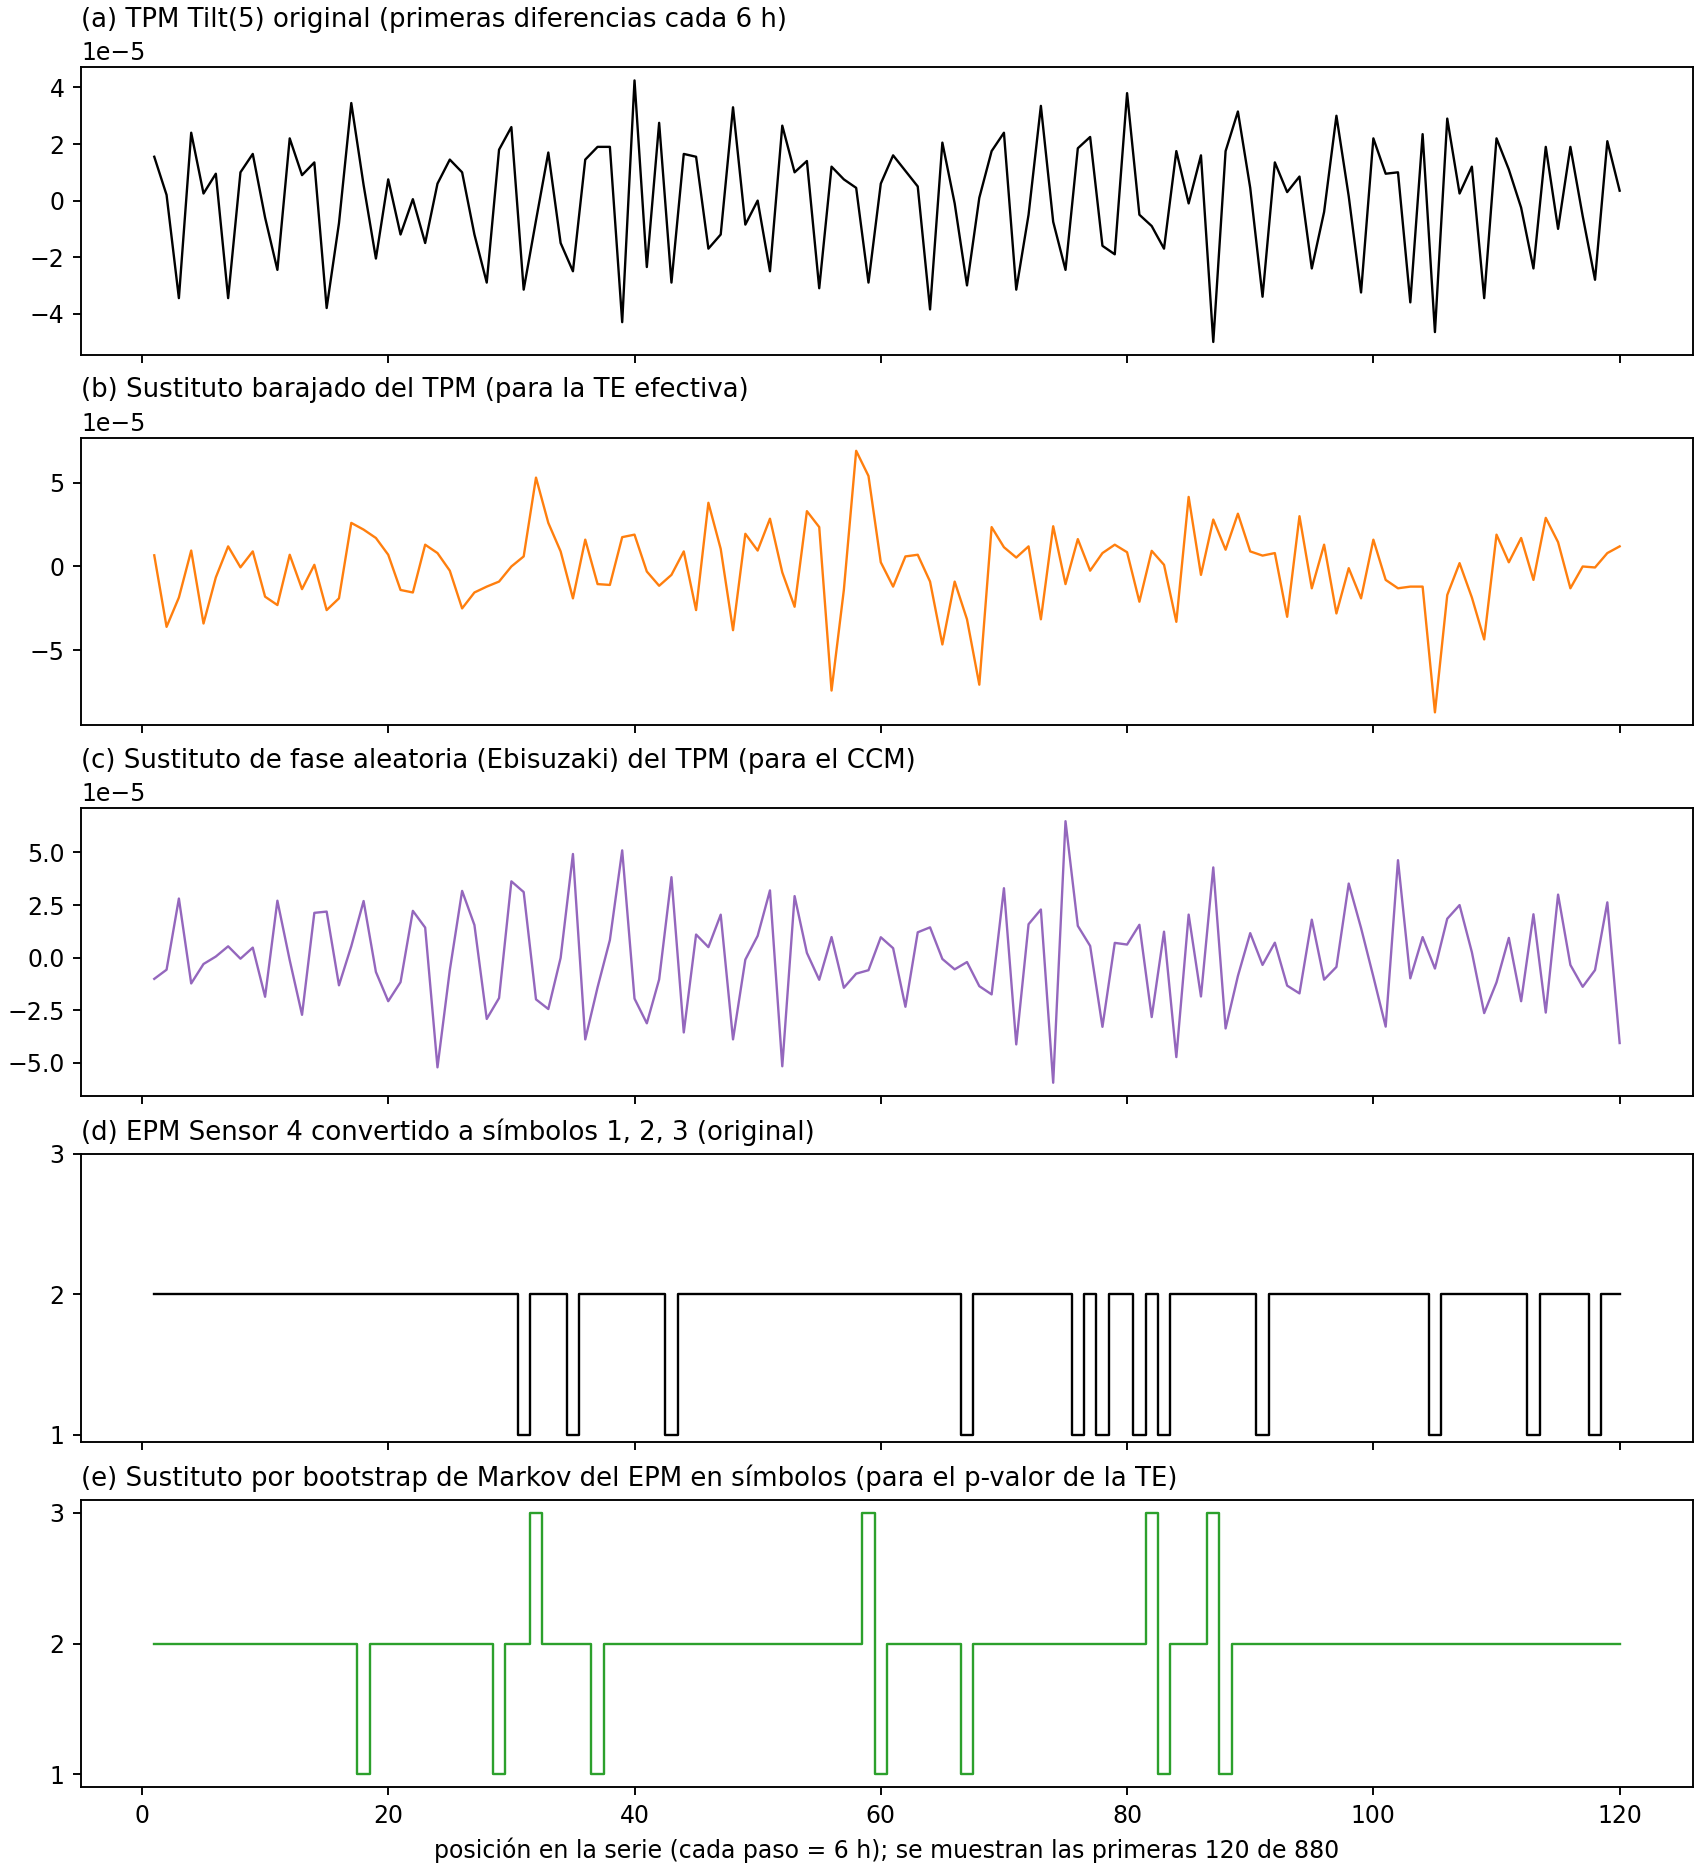
\includegraphics[width=0.92\textwidth]{sustitutos_ejemplo.png}
\caption{Cómo se ve cada sustituto, con datos reales (par Sensor 4 -- Tilt(5); primeras 120 de 880 posiciones). (a) Serie TPM original. (b) Un sustituto barajado del TPM, generado como lo hace RTransferEntropy (\texttt{sample} con reemplazo). (c) Un sustituto de fase aleatoria del TPM, generado con \texttt{pyEDM.SurrogateData(method='ebisuzaki')}, el que usa el CCM. (d) El EPM convertido a los símbolos 1, 2, 3. (e) Un sustituto del EPM generado con la función interna \texttt{markov\_boot\_step} de RTransferEntropy. Los programas que la generan están en \archivo{Guia\_TE\_CCM/figuras/}.}
\label{fig:sustitutos}
\end{figure}

\section{Sustituto 1: el barajado y la TE efectiva}

\subsection*{El problema: el estimador tiene sesgo}

Con pocos datos, la TE estimada sale mayor que cero aunque no haya ninguna relación. Es un error sistemático (sesgo) del estimador.

\begin{cita}{Behrendt et al.\ (2019), p.~2--3, sec.~2.2.}
The transfer entropy estimates are biased in small samples [20]. A bias correction is possible and used to calculate effective transfer entropy [20] as
\[ ET_{J\to I}(k,l) = T_{J\to I}(k,l) - T_{J_{\text{shuffled}}\to I}(k,l), \quad (5) \]
where $T_{J_{\text{shuffled}}\to I}(k,l)$ indicates the transfer entropy using a shuffled version of the time series J. Shuffling implies randomly drawing values from the observed time series J and realigning them to generate a new time series, which destroys the time series dependencies of J as well as the statistical dependencies between J and I. As a result, $T_{J_{\text{shuffled}}\to I}(k,l)$ converges to zero with increasing sample size and any nonzero value of $T_{J_{\text{shuffled}}\to I}(k,l)$ is due to small sample effects. To derive a consistent estimator, shuffling is repeated and the average of the resulting shuffled transfer entropy estimates across all replications serves as an estimator for the small sample bias, which is subsequently subtracted from the Shannon or Rényi transfer entropy estimate to obtain a bias corrected effective transfer entropy estimate.
\tcblower
\textbf{Traducción libre:} las estimaciones de TE tienen sesgo con muestras pequeñas. Se corrige calculando la TE efectiva (ecuación 5): la TE real menos la TE calculada con una versión barajada de $J$. Barajar es sacar valores al azar de la serie $J$ y ordenarlos en una serie nueva; eso destruye la dinámica de $J$ y su relación con $I$. Por eso la TE barajada tiende a cero cuando crece la muestra, y cualquier valor distinto de cero se debe al tamaño finito de la muestra. Se baraja varias veces, el promedio de las TE barajadas estima el sesgo, y se resta.
\end{cita}

La referencia [20] de Behrendt es Marschinski y Kantz (2002), Eur.\ Phys.\ J.\ B 30(2), 275--281. \textbf{No la hemos leído}; la conocemos a través de Behrendt.

\subsection*{Cómo se calcula, paso a paso}

Para un par (por ejemplo, Sensor 1 y POT(1)):
\begin{enumerate}
\item Calcular la TE real, TPM $\to$ EPM: $T = 0.0493$ bits.
\item Repetir 100 veces: barajar el TPM y calcular la TE con el TPM barajado.
\item Promediar esas 100 TE: es la estimación del sesgo.
\item Restar: TE efectiva $=$ TE real $-$ promedio barajado. El programa entregó $0.0424$ bits, así que el promedio barajado fue $0.0493 - 0.0424 = 0.0069$ bits.
\end{enumerate}

\begin{codigo}{RTransferEntropy 0.2.21, funciones \texttt{shuffle\_shannon} y \texttt{transfer\_entropy}.}
\begin{itemize}
\item El barajado es \texttt{sample(TPM, n, replace = TRUE)}: saca $n$ valores al azar del TPM \textbf{con reemplazo} (un valor puede salir dos veces). Coincide con ``randomly drawing values'' de Behrendt.
\item Solo se baraja la serie fuente (el TPM). El EPM queda intacto.
\item Si la TE efectiva sale negativa, el paquete la reporta como 0 (\texttt{pmax(0, ete)}). El artículo no lo menciona; es una decisión del código. Por eso 9 de los 56 pares TPM $\to$ EPM tienen TE efectiva exactamente 0.
\end{itemize}
\end{codigo}

\begin{cita}{Behrendt et al.\ (2019), p.~3.}
To calculate effective transfer entropy, the number of shuffles to be used has to be specified (default 100). To obtain reliable estimates, one should choose relatively large numbers.
\tcblower
\textbf{Traducción libre:} para la TE efectiva hay que fijar el número de barajados (por defecto 100). Para estimaciones confiables conviene un número relativamente grande.
\end{cita}

\begin{ojo}[Ojo: se usaron los 100 barajados por defecto]
El artículo recomienda ``números relativamente grandes'' sin dar una cifra. Usamos el valor por defecto. La TE efectiva solo se usa para describir la magnitud; \textbf{la significancia no depende de ella} (siguiente sección).
\end{ojo}

\section{Sustituto 2: el bootstrap de Markov y el p-valor}

\begin{cita}{Behrendt et al.\ (2019), p.~3.}
To assess the statistical significance of the transfer entropy estimates, as given by Eq. (3), we rely on a Markov block bootstrap [14]. In contrast to shuffling, it preserves the dependencies within the variables J and I, but eliminates the statistical dependencies between them. Repeated estimation of transfer entropy then provides the distribution of the estimates under the null hypothesis of no information flow. The associated p value is given by $1-\hat q_T$, where $\hat q_T$ denotes the quantile of the simulated distribution that is determined by the respective transfer entropy estimate.
\tcblower
\textbf{Traducción libre:} para evaluar la significancia de la TE usamos un bootstrap de bloques de Markov. A diferencia del barajado, conserva las dependencias dentro de cada serie, pero elimina la dependencia entre ellas. Repetir la estimación da la distribución de la TE bajo la hipótesis nula de ``no hay flujo de información''. El p-valor es $1-\hat q_T$, donde $\hat q_T$ es el cuantil de la distribución simulada en el que cae la TE real.
\end{cita}

\begin{cita}{Behrendt et al.\ (2019), p.~3.}
Statistical inference is based on bootstrap samples of the transfer entropy estimates, not the effective transfer entropy estimates. The number of bootstrap replications is set with nboot (default 300). The number of observations that are dropped from the beginning of the bootstrapped Markov chain is governed by burn (default 50).
\tcblower
\textbf{Traducción libre:} la inferencia se basa en el bootstrap de la TE, \textbf{no} de la TE efectiva. El número de réplicas es \texttt{nboot} (300 por defecto). El número de observaciones que se descartan al inicio de la cadena de Markov simulada es \texttt{burn} (50 por defecto).
\end{cita}

La referencia [14] de Behrendt es Dimpfl y Peter (2013), Stud.\ Nonlinear Dyn.\ Econom.\ 17(1), 85--102. \textbf{No la hemos leído.} El artículo de Behrendt no explica el algoritmo paso a paso; lo que sigue sale del código del paquete.

\begin{codigo}{RTransferEntropy 0.2.21, funciones \texttt{bootstrap\_shannon} y \texttt{markov\_boot\_step}.}
Para la dirección TPM $\to$ EPM, en cada una de las 300 réplicas:
\begin{enumerate}
\item Toma la serie EPM ya convertida en símbolos (1, 2, 3).
\item Estima sus probabilidades de transición de orden 1: por ejemplo, ``si ahora estoy en 2, ¿qué tan probable es que el siguiente sea 1, 2 o 3?'', contando en los datos.
\item Simula una cadena de Markov nueva con esas probabilidades: arranca en un símbolo al azar y en cada paso sortea el siguiente según las probabilidades estimadas. Genera $880 + 50$ símbolos y descarta los primeros 50 (\texttt{burn}).
\item Calcula la TE del TPM \textbf{original} hacia este EPM \textbf{simulado}.
\end{enumerate}
El EPM simulado tiene la misma dinámica de orden 1 que el real, pero se generó sin mirar el TPM. Por eso cualquier TE que salga es la que aparece \textbf{sin} flujo de información. Eso es la hipótesis nula.
\end{codigo}

\subsection*{El p-valor, con números reales}

\begin{codigo}{RTransferEntropy 0.2.21, función \texttt{transfer\_entropy}.}
El p-valor es \texttt{length(x[x > est]) / length(x)}: la fracción de las 300 réplicas cuya TE es \textbf{estrictamente mayor} que la TE real. Es lo mismo que $1-\hat q_T$ de Behrendt.
\end{codigo}

Ejemplos de nuestros resultados (dirección TPM $\to$ EPM):
\begin{center}\small
\begin{tabular}{llll}
\toprule
Par & Réplicas con TE mayor que la real & Cuenta & p-valor \\
\midrule
Sensor 3 -- POT(6) & 1 de 300 & $1/300$ & $0.0033$ \\
Sensor 2 -- POT(7) & 3 de 300 & $3/300$ & $0.0100$ \\
Sensor 3 -- Tilt(7) & 4 de 300 & $4/300$ & $0.0133$ \\
Sensor 3 -- Tilt(4) & 11 de 300 & $11/300$ & $0.0367$ \\
Sensor 1 -- POT(1) & 0 de 300 & $0/300$ & se reporta $<1/300$ \\
\bottomrule
\end{tabular}
\end{center}
La columna ``réplicas'' sale de multiplicar el p-valor del archivo \archivo{te\_resultados\_56\_pares.csv} por 300.

\begin{nota}[Nota: por qué ``$<1/300$'' y nunca ``0'']
Si ninguna de las 300 réplicas superó la TE real, el programa devuelve 0. Pero eso no significa que la probabilidad sea cero: con 300 réplicas no se pueden ver probabilidades menores que $1/300$. Lo correcto es decir $p < 1/300 \approx 0.0033$. Es el límite que describe Kugiumtzis (p.~11): el p-valor más pequeño posible es aproximadamente $1/(M+1)$.
\end{nota}

\section{Comparaciones múltiples: 56 pruebas a la vez}

\begin{nota}[Nota: el problema]
Con un umbral de $0.05$, una sola prueba se equivoca (dice ``significativo'' sin relación) con probabilidad $0.05$. Con 56 pruebas sin ninguna relación, se esperarían $56 \times 0.05 = 2.8$ pares ``significativos'' solo por azar.
\end{nota}

Una forma de controlar esto es la corrección de Benjamini--Hochberg, también llamada FDR (\emph{false discovery rate}, tasa de falsos descubrimientos). Kugiumtzis la describe y la usa:

\begin{cita}{Kugiumtzis (2013), p.~11.}
To account for multiple testing, the correction of false discovery rate (FDR) is employed [8]. According to FDR, we order the p-values of the $K(K-1)$ tests, $p_1 \le p_2 \le \dots \le p_{K(K-1)}$, and if $p_k$ is the largest p-value for which $p_k \le \alpha k/(K(K-1))$ holds, then all $H_0$ regarding $p_1,\dots,p_k$ are rejected at the significance level $\alpha$.
\tcblower
\textbf{Traducción libre:} para tener en cuenta las pruebas múltiples se usa la corrección FDR [8]. Se ordenan los p-valores de las $K(K-1)$ pruebas de menor a mayor; si $p_k$ es el mayor p-valor que cumple $p_k \le \alpha k / (K(K-1))$, se rechazan las hipótesis nulas de $p_1$ a $p_k$. (La referencia [8] es Benjamini y Hochberg, 1995.)
\end{cita}

En Kugiumtzis el número de pruebas es $K(K-1)$ porque compara $K$ variables entre sí. En nuestro caso el número de pruebas es $m = 56$, y la regla queda: $p_{(i)} \le i \times 0.05 / 56$.

\textbf{Cuenta con nuestros datos (TPM $\to$ EPM):}
\begin{enumerate}
\item Ordenados, los p-valores más pequeños son: nueve ceros ($<1/300$), dos de $0.0033$, uno de $0.0100$, uno de $0.0133$, uno de $0.0167$, uno de $0.0200$ y uno de $0.0367$.
\item Posición 12, $p_{(12)} = 0.0100$; umbral $12 \times 0.05/56 = 0.0107$. Como $0.0100 \le 0.0107$, cumple.
\item Posición 13, $p_{(13)} = 0.0133$; umbral $13\times0.05/56 = 0.0116$. No cumple. Las posiciones siguientes tampoco (por ejemplo, posición 14: $0.0167 > 0.0125$).
\item El mayor $k$ que cumple es 12, así que se rechazan las 12 primeras.
\end{enumerate}
\textbf{Resultado: 12 pares significativos tras Benjamini--Hochberg.}

\begin{nota}[Nota: los ceros no cambian el resultado]
Si los nueve ceros fueran en realidad $1/300 = 0.0033$, el resultado sería el mismo, porque la regla solo mira el mayor $k$ que cumple, y $p_{(12)} = 0.0100$ sigue cumpliendo.
\end{nota}

% =====================================================================
\chapter{Resultados de la TE y cómo se obtuvieron}\label{cap:res-te}

\section{La cadena de programas}

\begin{center}\small
\begin{tabular}{>{\raggedright}p{4.2cm}>{\raggedright}p{4.2cm}>{\raggedright\arraybackslash}p{5.6cm}}
\toprule
Programa (en \archivo{Códigos/TE\_R/}) & Entrada & Salida \\
\midrule
\texttt{preparar\_datos.py} & \texttt{Data\_limpia\_completa/}\allowbreak\texttt{*.csv} & \texttt{data/}\allowbreak\texttt{series\_diferencias\_6h.csv} \\
\texttt{te\_56\_pares.R} (unos 4 min) & el archivo anterior & \texttt{data/te\_resultados\_56\_pares.csv} \\
\texttt{graficar\_resultados.py} & el archivo anterior & \texttt{figuras/te\_valores\_heatmap.png}, \texttt{figuras/te\_pvalor\_heatmap.png} \\
\bottomrule
\end{tabular}
\end{center}

\texttt{graficar\_resultados.py} no calcula nada: solo dibuja los números que entregó el paquete.

\section{Figura 1: TE real y TE efectiva}

\begin{figure}[ht]
\centering
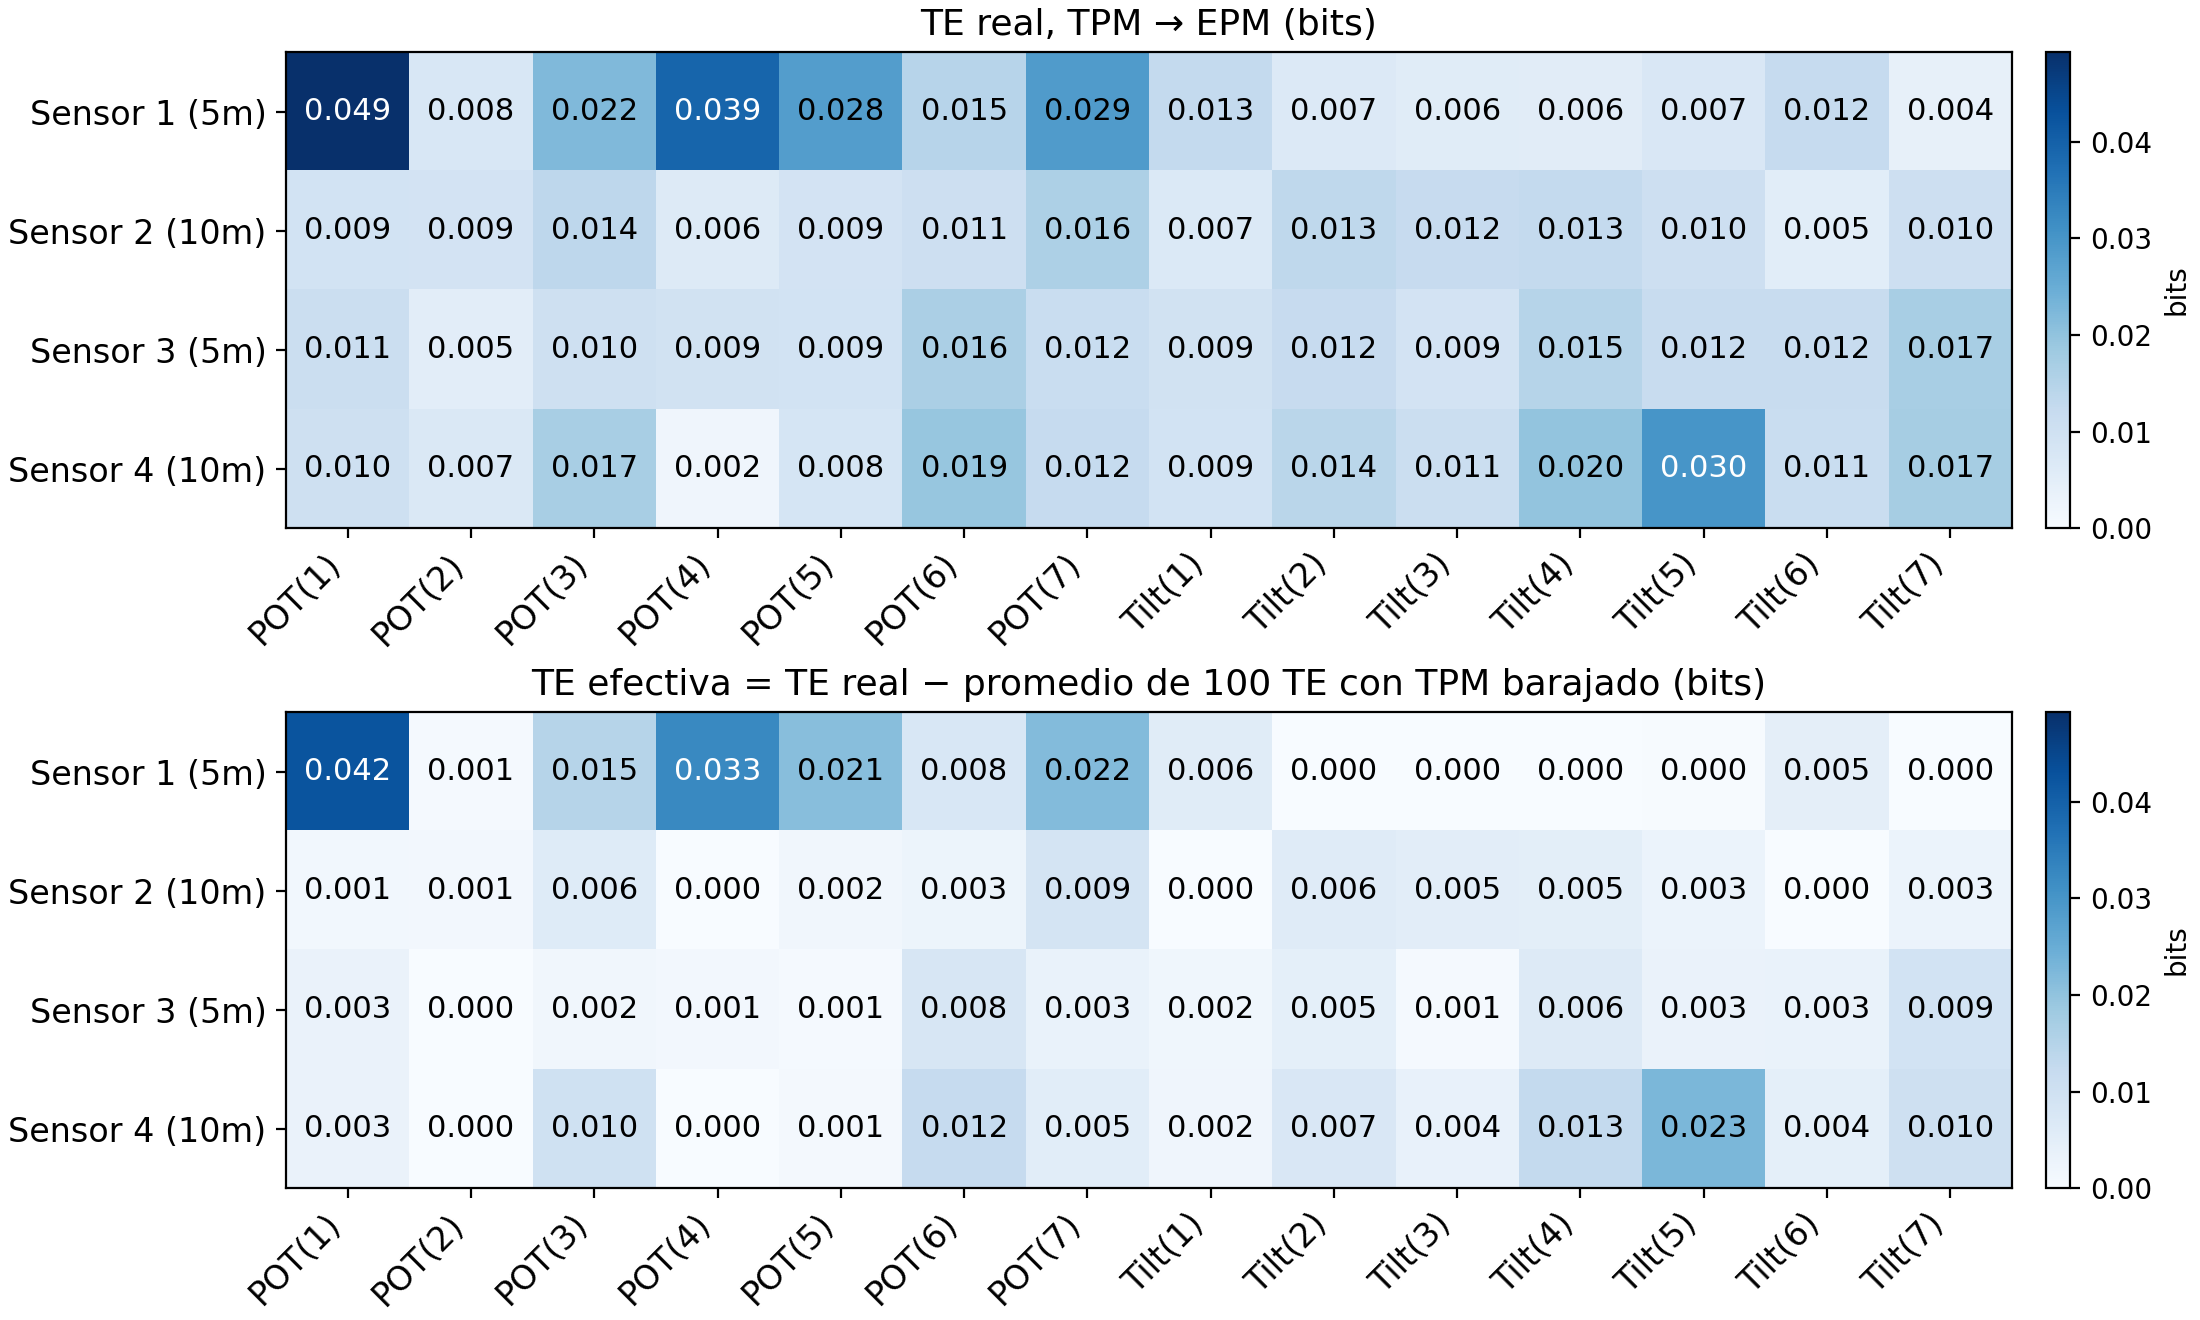
\includegraphics[width=\textwidth]{te_valores_heatmap.png}
\caption{Arriba: TE real, TPM $\to$ EPM, en bits. Abajo: TE efectiva (TE real menos el promedio de 100 TE con el TPM barajado). Filas: los 4 sensores EPM. Columnas: las 14 series TPM. Cada casilla es un par. Las dos partes usan la misma escala de color, de 0 al máximo de la TE real.}
\label{fig:te-valores}
\end{figure}

\textbf{Cómo leerla}: la casilla de la fila ``Sensor 1 (5m)'' y la columna ``POT(1)'' dice $0.049$ arriba y $0.042$ abajo: la TE real de POT(1) hacia el Sensor 1 es $0.049$ bits, y quitando el sesgo queda $0.042$ bits. Es el valor más alto de los 56.

\textbf{Lo que muestra}: la TE real va de $0.002$ a $0.049$ bits. En 9 pares la TE efectiva es 0, es decir, la TE real no superó el promedio de los barajados.

\section{Figura 2: p-valores}

\begin{figure}[ht]
\centering
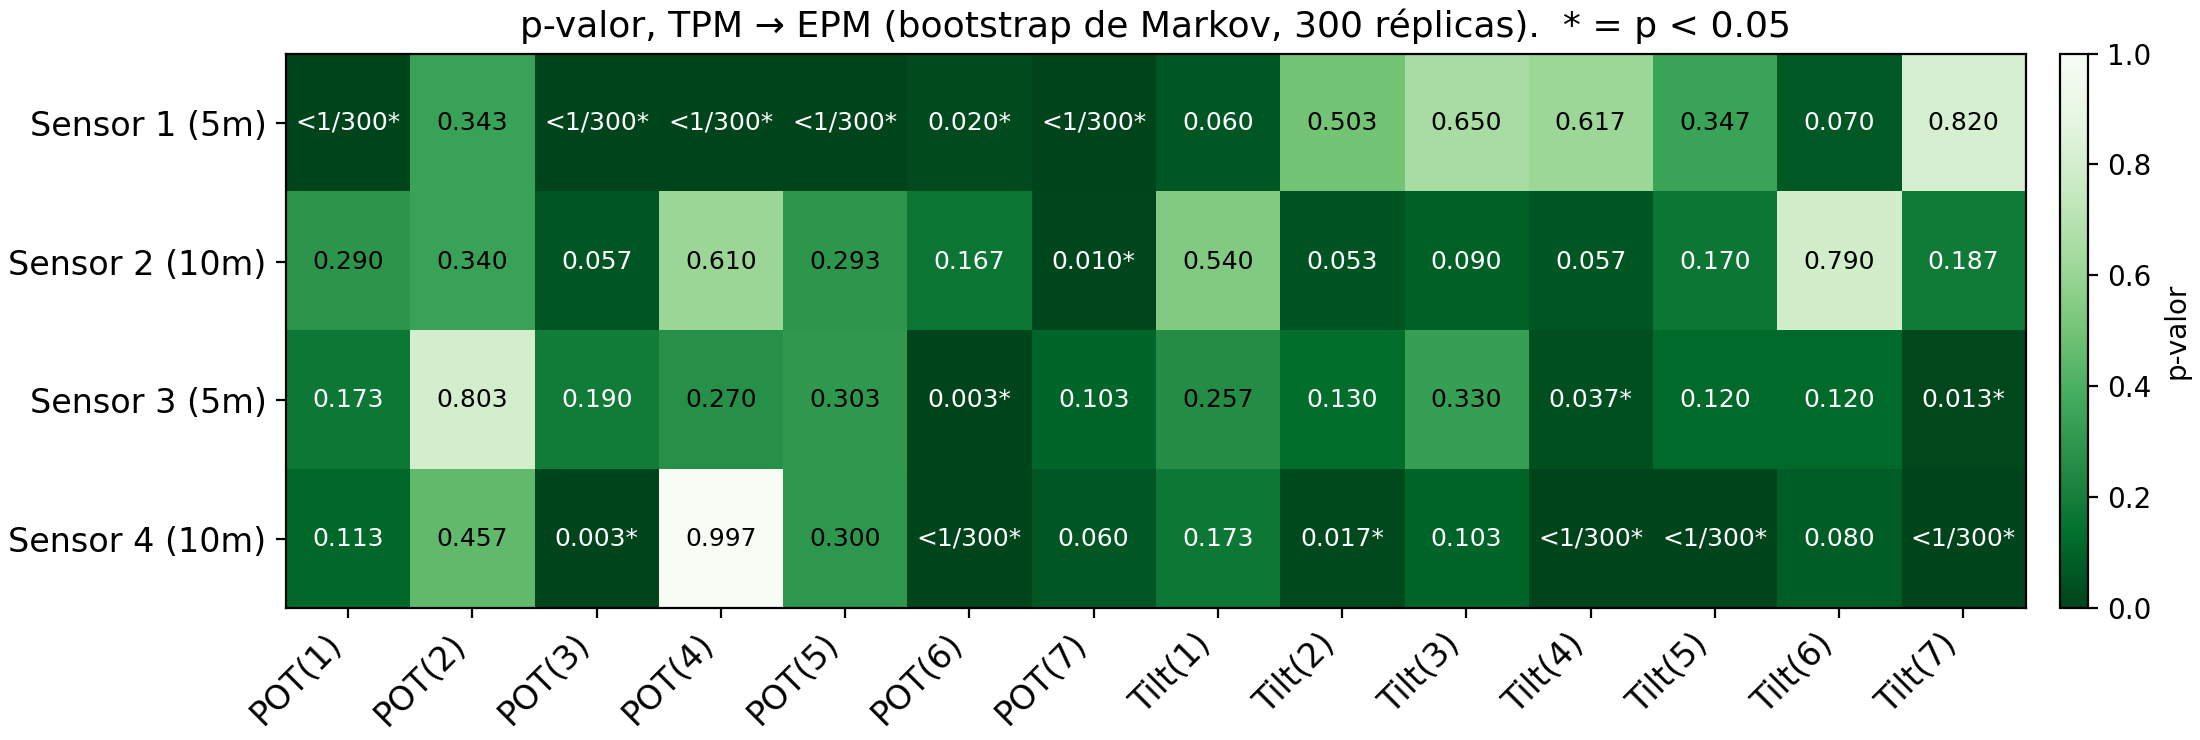
\includegraphics[width=\textwidth]{te_pvalor_heatmap.png}
\caption{p-valor de cada par, TPM $\to$ EPM, por bootstrap de Markov con 300 réplicas. ``$<$1/300'' significa que ninguna réplica superó la TE real. El asterisco marca $p < 0.05$. Color más oscuro = p más pequeño.}
\label{fig:te-p}
\end{figure}

\textbf{Resultado}: 16 de 56 pares tienen $p < 0.05$ en la dirección TPM $\to$ EPM. Por azar se esperarían 2.8. Con Benjamini--Hochberg quedan 12. En la dirección contraria (EPM $\to$ TPM) hay 12 con $p<0.05$ y 5 tras Benjamini--Hochberg.

\section{Tabla: los 16 pares con $p < 0.05$}

\begin{center}\small
\begin{tabular}{llcccc}
\toprule
EPM & TPM & TE (bits) & TE efectiva (bits) & p-valor & Pasa BH \\
\midrule
Sensor 1 (5m) & POT(1) & 0.0493 & 0.0424 & $<1/300$ & sí \\
Sensor 1 (5m) & POT(4) & 0.0392 & 0.0325 & $<1/300$ & sí \\
Sensor 1 (5m) & POT(7) & 0.0285 & 0.0218 & $<1/300$ & sí \\
Sensor 1 (5m) & POT(5) & 0.0283 & 0.0211 & $<1/300$ & sí \\
Sensor 1 (5m) & POT(3) & 0.0221 & 0.0148 & $<1/300$ & sí \\
Sensor 1 (5m) & POT(6) & 0.0145 & 0.0077 & 0.0200 & no \\
Sensor 2 (10m) & POT(7) & 0.0160 & 0.0086 & 0.0100 & sí \\
Sensor 3 (5m) & Tilt(7) & 0.0168 & 0.0091 & 0.0133 & no \\
Sensor 3 (5m) & POT(6) & 0.0164 & 0.0080 & 0.0033 & sí \\
Sensor 3 (5m) & Tilt(4) & 0.0147 & 0.0064 & 0.0367 & no \\
Sensor 4 (10m) & Tilt(5) & 0.0299 & 0.0226 & $<1/300$ & sí \\
Sensor 4 (10m) & Tilt(4) & 0.0198 & 0.0126 & $<1/300$ & sí \\
Sensor 4 (10m) & POT(6) & 0.0193 & 0.0122 & $<1/300$ & sí \\
Sensor 4 (10m) & Tilt(7) & 0.0173 & 0.0101 & $<1/300$ & sí \\
Sensor 4 (10m) & POT(3) & 0.0169 & 0.0100 & 0.0033 & sí \\
Sensor 4 (10m) & Tilt(2) & 0.0141 & 0.0074 & 0.0167 & no \\
\bottomrule
\end{tabular}
\end{center}
Todos los valores salen de \archivo{TE\_R/data/te\_resultados\_56\_pares.csv}, redondeados a 4 decimales. ``Pasa BH'' es la corrección de Benjamini--Hochberg al 5\,\% sobre los 56 p-valores.

\section{¿Cómo se interpreta?}

\begin{itemize}
\item \textbf{Lo que sí se puede decir}: en 16 pares (12 con la corrección), la TE observada es mayor que la que aparece cuando el EPM se simula sin relación con el TPM. Es decir, en esos pares el pasado del TPM sí aporta información sobre el siguiente valor del EPM, más allá de su propio pasado.
\item \textbf{Lo que no se puede decir}: que el TPM \emph{cause} físicamente el EPM (Schreiber p.~4, causa común; Yuan y Shou p.~9). Tampoco que en los otros 40 pares no hay relación (Theiler, PDF p.~14: no rechazar es no concluyente).
\item \textbf{Sobre el tamaño}: no hay una escala absoluta de ``TE grande'':
\end{itemize}

\begin{cita}{Behrendt et al.\ (2019), p.~5.}
Since the transfer entropy is not normalized to a certain interval, it is clear that the information flow in both directions cannot be compared across different quantiles but only for the same quantiles, i.e. determining the dominant direction of the information flow is not possible across different quantile choices.
\tcblower
\textbf{Traducción libre:} como la TE no está normalizada a un intervalo, el flujo de información en ambas direcciones no se puede comparar entre distintas elecciones de cuantiles, solo con los mismos cuantiles.
\end{cita}

Como referencia: en el ejemplo no lineal de Behrendt (tabla 2, p.~5) la TE es $0.0125$ bits, con TE efectiva $0.0115$ y $p = 0.0000$, y los autores la reportan como un flujo significativo. Es otra serie y otro tamaño de muestra, así que solo sirve para mostrar que valores de centésimas de bit no son raros. \textbf{No sirve para comparar magnitudes.}

% =====================================================================
\chapter{Convergent cross mapping (CCM)}\label{cap:ccm}

\section{La idea, en palabras}

\begin{cita}{Deyle et al.\ (2016), p.~13082 (PDF p.~2).}
It looks for signatures of the cause in the time series of the affected variable. The idea is that if a variable, X, can predict the current or previous state of another variable, Y, then Y causally influenced X. For example, if sardine abundance can be used to recover sea surface temperature, then temperature had a causal effect on sardines.
\tcblower
\textbf{Traducción libre:} el CCM busca huellas de la causa en la serie de la variable afectada. Si una variable $X$ puede predecir el estado actual o anterior de otra variable $Y$, entonces $Y$ influyó causalmente en $X$. Por ejemplo, si con la abundancia de sardinas se puede recuperar la temperatura del mar, la temperatura tuvo un efecto causal sobre las sardinas.
\end{cita}

\begin{cita}{Yuan y Shou (2020), p.~11, líneas 274--276.}
We note that there is a striking contrast between Granger causality and SSR: Whereas in Granger causality the history of a causer can predict the future of its causee, in SSR the history of a causee can estimate the current value of its causer.
\tcblower
\textbf{Traducción libre:} hay un contraste llamativo entre la causalidad de Granger y la reconstrucción del espacio de estados (SSR): en Granger, la historia de la causa predice el futuro del efecto; en SSR, la historia del efecto estima el valor actual de la causa.
\end{cita}

\textbf{La dirección es al revés de lo que se esperaría}, y es la confusión más común:
\begin{itemize}
\item \textbf{TE}: el pasado del TPM ayuda a predecir el EPM $\Rightarrow$ evidencia de TPM $\to$ EPM.
\item \textbf{CCM}: la historia del EPM permite estimar el TPM $\Rightarrow$ evidencia de TPM $\to$ EPM.
\end{itemize}
En el CCM, con los vectores construidos a partir del EPM se estima el TPM. Si se puede, el TPM dejó huella en el EPM.

\section{Paso 1: vectores de retardo}

\begin{nota}[Nota: vector de retardo, $E$ y $\tau$]
Con la serie EPM, en cada tiempo $t$ se arma el vector
\[ \big[\,\text{EPM}(t),\ \text{EPM}(t-\tau),\ \text{EPM}(t-2\tau),\ \dots,\ \text{EPM}(t-(E-1)\tau)\,\big]. \]
\begin{itemize}
\item $E$ es la \textbf{dimensión}: cuántos valores tiene el vector.
\item $\tau$ es el \textbf{retardo}: cada cuántos pasos se toma un valor. Con $\tau = 1$ se toman valores consecutivos (cada 6 h en nuestros datos).
\end{itemize}
El conjunto de todos esos vectores es el \textbf{espacio de retardos} del EPM (Yuan y Shou dicen \emph{delay space}). Cada vector es un punto en un espacio de $E$ dimensiones.
\end{nota}

Ejemplo: con $E = 3$ y $\tau = 1$, el vector en el tiempo $t$ es $[\text{EPM}(t), \text{EPM}(t-1), \text{EPM}(t-2)]$: el valor actual y los dos anteriores.

\section{Paso 2: la habilidad de cross-map $\rho$}

\begin{cita}{Yuan y Shou (2020), p.~14, figura 8(A).}
Consider X(T) denoted by the red dot (“actual X(T)” in 1), which we want to predict from Y delay vectors. We first look up the contemporaneous Y delay vector ([Y(T), Y(T - 1), Y(T - 2)]) (red dynamics in 2), and identify times within our training data when delay vectors of Y were the most similar to our red delay vector (blue segments 3). We then look up their contemporaneous values of X (4, blue crosses), and use their weighted average to predict X(T) (5, open magenta circle). We repeat this procedure for many choices of X(T) and calculate the Pearson correlation between the actual values of X(T) and our predicted values of X(T) (6). This correlation is called the “cross map skill”.
\tcblower
\textbf{Traducción libre:} para predecir $X(T)$ con vectores de $Y$: (1) se toma el vector de $Y$ en el mismo tiempo $T$; (2) se buscan en los datos de entrenamiento los tiempos en que los vectores de $Y$ más se parecían a ese; (3) se miran los valores de $X$ en esos tiempos; (4) su promedio ponderado es la predicción de $X(T)$. Se repite para muchos $T$ y se calcula la correlación de Pearson entre los $X$ reales y los predichos. Esa correlación es la ``habilidad de cross-map''.
\end{cita}

En nuestro caso, $Y$ de la cita es el EPM (el efecto) y $X$ es el TPM (la posible causa).

\begin{codigo}{pyEDM 2.5.7, \texttt{Simplex} (proyección simplex).}
\begin{itemize}
\item Número de vecinos: $E+1$ (el valor por defecto que fija el programa cuando no se le da otro).
\item Peso de cada vecino: $w_i = \exp(-d_i/d_1)$, donde $d_i$ es la distancia del vecino $i$ y $d_1$ la del vecino más cercano. El vecino más cercano pesa $e^{-1}$; los más lejanos pesan menos.
\item Predicción: $\hat X(T) = \sum_i w_i X(t_i) \big/ \sum_i w_i$.
\item \emph{Leave-one-out}: para predecir el tiempo $T$ se usan todos los demás tiempos, menos el propio $T$.
\end{itemize}
El método de proyección simplex es de Sugihara y May (1990), citado por Deyle et al.\ (ref.~22). \textbf{Ese artículo no está en tu carpeta}; la fórmula de los pesos la tomé del código de pyEDM.
\end{codigo}

\section{Paso 3: elegir $E$ y $\tau$}

\begin{cita}{Yuan y Shou (2020), p.~21, líneas 517--534 (extracto).}
Convergent cross mapping looks for a delay map from X to Y. [\dots] Thus in order to apply CCM one needs to choose the delay $\tau$ and the vector length (dimension of the delay space) E. [\dots] There are different ways to do this, but no method is obviously best ([19, 31]). Following [19] and [60] we chose $\tau$ and E to maximize univariate one-step-ahead forecast of the putative causee X. [\dots] As per the field standard, we used leave-one-out cross-validation to do simplex projection. [\dots] We performed a grid search, varying $\tau$ from 1 to 6 and varying E from 1 to 6. We then used the combination of $\tau$ and E that maximized the forecast skill (the Pearson correlation between forecasts and true values) for subsequent CCM analysis.
\tcblower
\textbf{Traducción libre:} el CCM busca un mapa desde el espacio de retardos del efecto hacia la causa. Hay que escoger $\tau$ y $E$. No hay un método claramente mejor. Siguiendo a [19] y [60], se escogen los que maximizan el pronóstico a un paso del supuesto efecto, con proyección simplex y \emph{leave-one-out}. Se prueba una rejilla de $\tau$ de 1 a 6 y $E$ de 1 a 6, y se usa la combinación con mayor habilidad de pronóstico (correlación de Pearson entre pronósticos y valores reales).
\end{cita}

Ojo con las letras: en esta cita de los Métodos, $X$ es el \textbf{efecto} (en la figura 8 era al revés). En nuestro caso, el efecto es el EPM. Por eso $E$ y $\tau$ se escogen con el EPM solo.

\textbf{Resultado} (archivo \archivo{CCM\_py/data/ccm\_E\_tau\_por\_sensor.csv}):
\begin{center}\small
\begin{tabular}{lccc}
\toprule
Sensor EPM & $E$ & $\tau$ & Habilidad de pronóstico a un paso \\
\midrule
Sensor 1 (5m) & 6 & 1 & 0.517 \\
Sensor 2 (10m) & 5 & 1 & 0.499 \\
Sensor 3 (5m) & 3 & 1 & 0.481 \\
Sensor 4 (10m) & 3 & 1 & 0.281 \\
\bottomrule
\end{tabular}
\end{center}
Ejemplo de lectura: para el Sensor 1, de las 36 combinaciones ($6 \times 6$), la mejor fue $E = 6$, $\tau = 1$, y con ella la correlación entre el pronóstico a un paso y el valor real fue 0.517.

\section{Los cuatro criterios del CCM}

\begin{cita}{Yuan y Shou (2020), p.~14, líneas 335--344.}
Four criteria have been proposed to infer causality [60, 74, 19] (Fig 8B): First, the cross map skill must be positive. That is, when using the causee delay space to predict the causer, the Pearson correlation coefficient between true values and predictions must be positive. Second, the cross map skill must be significant. That is, the cross map skill must be greater than the “null” cross map skill when the putative causer is replaced with “surrogate data” (a type of null model discussed toward the end of this article). Third, the cross map skill must increase with an increasing amount of training data. Last, cross map skill must be greater when predicting past values of causer than when predicting future values of causer (the “prediction lag” test; [74, 19]). This test was proposed to overcome the strong forcing failure mode (the second row of Fig 7). However, see Appendix 1.12 for problems that we have found using this criterion. In practice, many CCM analyses use only a subset of these four criteria [60, 76, 77, 78].
\tcblower
\textbf{Traducción libre:} se han propuesto cuatro criterios: (1) la habilidad de cross-map debe ser positiva; (2) debe ser significativa, es decir, mayor que la habilidad ``nula'' obtenida al reemplazar la posible causa por datos sustitutos; (3) debe crecer con la cantidad de datos de entrenamiento; (4) debe ser mayor al predecir valores pasados de la causa que valores futuros (prueba del rezago de predicción). Esta última se propuso para el modo de falla de ``forzamiento fuerte'', pero los autores encontraron problemas con ella. En la práctica, muchos análisis usan solo algunos de los cuatro criterios.
\end{cita}

Las referencias [60], [74] y [19] son Sugihara et al.\ (2012), Ye et al.\ (2015) y Cobey y Baskerville (2016). \textbf{No las hemos leído}; los criterios los tomamos tal como los resume Yuan y Shou.

El criterio~2 es el de los sustitutos y tiene su propio capítulo (\ref{cap:sust-ccm}). Los otros tres:

\subsection*{Criterio 1: $\rho > 0$}
Se calcula $\rho$ con todos los datos (\emph{leave-one-out}) y se exige $\rho > 0$.

\subsection*{Criterio 3: convergencia (procedimiento alternativo de Kendall)}

\begin{cita}{Yuan y Shou (2020), p.~22, líneas 572--582.}
For “alternative” CCM testing, we only changed how the third CCM criterion (cross map skill increases with more training data) were tested. Here, instead of using the bootstrap test of [19], we tested the third CCM criterion using Kendall’s $\tau$ test as suggested in [81]. To do this, we varied the library size from a minimum of 15 vectors to the the maximum library size ($200-(E-1)\tau-1$), in increments of 3 vectors. For each library size, we computed cross map skill using 50 libraries randomly sampled without replacement (e.g. the 50 libraries would be identical at the maximal library size). We then computed the median cross map skill for each library size. Finally we ran a 1-tailed Kendall’s $\tau$ test for a positive association between library size and median cross map skill. We used the function stats.kendalltau from the Python package SciPy to compute a 2-tailed p-value, and then divided this p-value by 2 to get a 1-tailed p-value. We said that cross map skill increased with training data if the $\tau$ statistic was positive and the 1-tailed p-value was $\le 0.05$.
\tcblower
\textbf{Traducción libre:} en la versión ``alternativa'' el criterio 3 se prueba con la prueba $\tau$ de Kendall. Se varía el tamaño de la biblioteca desde 15 vectores hasta el máximo, de 3 en 3. Para cada tamaño se calcula la habilidad con 50 bibliotecas sacadas al azar sin reemplazo, y se toma la mediana. Se hace una prueba de Kendall de una cola para ver si la mediana crece con el tamaño (p de dos colas de SciPy dividido entre 2). Pasa si el estadístico es positivo y el p de una cola es $\le 0.05$.
\end{cita}

\begin{nota}[Nota: biblioteca y $\tau$ de Kendall]
\begin{itemize}
\item La \textbf{biblioteca} es el conjunto de vectores de retardo entre los que se buscan los vecinos. Si el CCM refleja una relación real, más biblioteca debería dar vecinos más parecidos y mejor $\rho$. Eso es la ``convergencia''.
\item El \textbf{$\tau$ de Kendall} (no confundir con el retardo $\tau$) mide si dos cantidades suben juntas: vale $+1$ si siempre que crece una crece la otra, y $-1$ si siempre que crece una baja la otra.
\end{itemize}
\end{nota}

En nuestro caso, 200 se reemplaza por 880: el tamaño máximo es $880 - (E-1)\tau - 1$. Con $E=6$, $\tau = 1$ (Sensor 1), es $880 - 5 - 1 = 874$ vectores.

\subsection*{Criterio 4: no se usa}

\begin{cita}{Yuan y Shou (2020), p.~21, líneas 545--547.}
We did not use the fourth criterion (the prediction lag test) since its interpretation is unclear for periodic systems (Fig 19).
\tcblower
\textbf{Traducción libre:} no usamos el cuarto criterio (la prueba del rezago), porque su interpretación no es clara en sistemas periódicos.
\end{cita}

En su apéndice 1.12 (p.~42--44) muestran que esa prueba da falsos negativos, falsos positivos y resultados poco claros con forzantes periódicos.

\textbf{Un par ``pasa el CCM''} si cumple los criterios 1, 2 y 3.

\section{Advertencias de los propios autores}

\begin{cita}{Yuan y Shou (2020), p.~11, líneas 288--292.}
It is commonly thought that the use of SSR to detect causality is justified by theorems from Takens [58] and Sauer et al. [59]. However, these theorems state the conditions under which continuous delay maps are likely (but not quite guaranteed) to arise. They do not show (or even suggest) that the existence of a continuous delay map implies a causal relationship.
\tcblower
\textbf{Traducción libre:} se suele pensar que el teorema de Takens justifica usar SSR para detectar causalidad. Pero esos teoremas dicen cuándo es probable que exista un mapa continuo de retardos; no muestran (ni sugieren) que la existencia de ese mapa implique una relación causal.
\end{cita}

\begin{cita}{Yuan y Shou (2020), p.~15, líneas 362--363 y 365--371.}
Unlike in linear Granger causality, there is no standard and automatic test procedure for CCM causality criteria [19, 24]. [\dots] Although Granger causality and CCM can perform well when requirements are met, both are highly sensitive to the levels of process and measurement noise [\dots]. CCM is additionally sensitive to test procedure details.
\tcblower
\textbf{Traducción libre:} a diferencia de la causalidad de Granger lineal, no hay un procedimiento estándar y automático para los criterios del CCM. Granger y CCM funcionan bien si se cumplen sus requisitos, pero ambos son muy sensibles al ruido del proceso y de medición. El CCM además es sensible a los detalles del procedimiento.
\end{cita}

\begin{cita}{Yuan y Shou (2020), p.~11 y 13, líneas 305--308 y 314--316.}
The second row of Fig 7 shows a failure mode where a continuous delay map appears in both directions even though the causal relationship is only unidirectional. This has been called “strong forcing” or “synchrony” [60] [\dots]. In the third row of Fig 7, the oscillation period of X is an integer multiple of that of Y [\dots]. A continuous delay map exists from X to Z, but not from Z to X, even if X and Z are causally unrelated.
\tcblower
\textbf{Traducción libre:} un modo de falla es el ``forzamiento fuerte'' o ``sincronía'': aparece un mapa en las dos direcciones aunque la causalidad vaya en una sola. Otro: si el período de oscilación de una serie es múltiplo entero del de otra, puede aparecer un mapa aunque las dos no tengan relación causal.
\end{cita}

% =====================================================================
\chapter{Los sustitutos del CCM}\label{cap:sust-ccm}

\section{El criterio 2, tal como lo describen Yuan y Shou}

\begin{cita}{Yuan y Shou (2020), p.~21--22, líneas 555--563.}
The second CCM criterion is that the cross map skill from causee to causer with real data must be greater than the cross map skill when the putative causer is replaced with surrogate data. To test this criterion, we first computed cross map skill using the same training and testing time points as before to obtain a single cross map skill value. We then repeatedly (1000 times) computed cross map skill in the same way, but now with the putative causer time series replaced with random phase surrogate data. Random phase surrogate data were generated by Ebisuzaki’s method as implemented in the rEDM function make\_surrogate\_data. We computed the significance p-value as the fraction of cross map skill values obtained with surrogate time series that were equal to or greater than the cross map skill value obtained with the original putative causer time series. A putative causal link passed this criterion if the p-value was less than or equal to 0.05.
\tcblower
\textbf{Traducción libre:} el criterio 2 exige que la habilidad de cross-map con datos reales sea mayor que la obtenida al reemplazar la posible causa por sustitutos. Primero se calcula la habilidad real. Luego se repite 1000 veces reemplazando la posible causa por sustitutos de fase aleatoria (método de Ebisuzaki, implementado en rEDM). El p-valor es la fracción de sustitutos con habilidad igual o mayor que la real. El vínculo pasa si $p \le 0.05$.
\end{cita}

\textbf{Paso a paso en nuestro caso, para un par EPM--TPM:}
\begin{enumerate}
\item Calcular $\rho_{\text{real}}$: el espacio de retardos del EPM estima el TPM real.
\item Generar 1000 sustitutos de fase aleatoria del \textbf{TPM}. El EPM no se toca.
\item Para cada sustituto, calcular $\rho$ con el mismo EPM, el mismo $E$ y el mismo $\tau$.
\item $p = $ (número de sustitutos con $\rho \ge \rho_{\text{real}}$) $/ 1000$.
\item Pasa si $p \le 0.05$. Si ningún sustituto alcanza a $\rho_{\text{real}}$, se reporta $p < 1/1000$.
\end{enumerate}

\section{Qué es un sustituto de fase aleatoria}

\begin{cita}{Yuan y Shou (2020), p.~45, figura 21.}
Surrogate data methods test the significance of this causal signal by comparing it to causal signals generated when one of the time series (Y) is replaced by a similar time series ($Y_{\text{surr}}$) which is assumed to be causally independent of X. Random phase surrogate data methods generate $Y_{\text{surr}}$ by representing Y as a sum of sine waves (upper left), randomly shifting the phases of the component sine waves (upper right green), and summing up the shifted sine waves (lower right green). A p-value is calculated as the fraction of $(X, Y_{\text{surr}})$ time series that produce a causal signal that is at least as strong as the causal signal from the original $(X, Y)$ time series.
\tcblower
\textbf{Traducción libre:} los métodos de sustitutos prueban la significancia comparando la señal causal real con la que se obtiene al reemplazar una serie por otra parecida que se supone independiente. Los de fase aleatoria representan la serie como suma de ondas seno, desplazan al azar la fase de cada onda y las vuelven a sumar. El p-valor es la fracción de pares (serie, sustituto) que dan una señal al menos tan fuerte como la original.
\end{cita}

\begin{codigo}{pyEDM 2.5.7, \texttt{SurrogateData(method='ebisuzaki')}.}
\begin{enumerate}
\item Calcula la transformada de Fourier del TPM y guarda las amplitudes (el espectro). Pone en 0 la amplitud de frecuencia cero, que corresponde a la media.
\item Sortea una fase uniforme entre 0 y $2\pi$ para cada frecuencia, y la refleja con signo opuesto en la mitad simétrica para que el resultado sea real.
\item Invierte la transformada y reescala el resultado para que tenga la misma desviación estándar que el TPM original.
\end{enumerate}
Es el mismo esquema del Algoritmo I de Theiler (PDF p.~7--8). El método se atribuye a Ebisuzaki (1997, \emph{Journal of Climate}), que \textbf{no está en tu carpeta}.
\end{codigo}

\section{Por qué fase aleatoria y no barajado}

\begin{itemize}
\item \textbf{Barajar destruye la dependencia temporal} (Yuan y Shou, p.~15, líneas 388--389). El barajado compara contra una serie sin memoria, que es una nula demasiado fácil de rechazar. En el experimento de Yuan y Shou (figura 10, p.~17), barajar da 29.5\,\% de falsos positivos contra 5\,\% de la fase aleatoria.
\item \textbf{La fase aleatoria conserva el espectro} y con él la autocorrelación (Yuan y Shou, p.~17, líneas 396--397). La nula es: ``el TPM es una serie con la misma memoria que la real, pero sin relación con el EPM''.
\item \textbf{Es lo que hacen Yuan y Shou} en sus criterios del CCM (p.~21--22).
\end{itemize}

\section{Lo que la fase aleatoria no resuelve: ciclos compartidos}

\begin{cita}{Yuan y Shou (2020), p.~17, líneas 397--399.}
The random phase test thus assumes that the power spectrum of each time series does not depend on the presence of a causal relationship.
\tcblower
\textbf{Traducción libre:} la prueba de fase aleatoria supone que el espectro de potencia de cada serie no depende de que haya una relación causal.
\end{cita}

Deyle et al.\ (2016) enfrentaron un problema parecido: la gripe y el clima tienen el mismo ciclo anual. Para eso usaron otro sustituto:

\begin{cita}{Deyle et al.\ (2016), p.~13086 (PDF p.~6), Métodos.}
For a forcing variable Z(t) (e.g., absolute humidity or temperature), we calculate the day of year average Z (i.e., the seasonal cycle) as earlier, and the seasonal anomaly as the difference between the observed value Z(t) and the day of year average for that day [\dots]. We then randomly shuffle (permute) the time indices of the seasonal anomalies. Adding the shuffled anomalies back to the season average gives a surrogate time series Z* that has the same seasonal average as Z, but with random anomalies. If Z is in fact a driver of influenza, then influenza will be sensitive not only to the seasonal component of Z but also to the anomalies. Thus, influenza should better predict the real time series Z than the surrogate Z*. In practice, we repeat the shuffling procedure 500 times to produce an ensemble of surrogates.
\tcblower
\textbf{Traducción libre:} para la posible causa $Z(t)$ se calcula el promedio por día del año (el ciclo estacional) y la anomalía (valor observado menos ese promedio). Se barajan las anomalías y se suman de nuevo al ciclo: el sustituto $Z^*$ tiene el mismo ciclo que $Z$, pero anomalías al azar. Si $Z$ de verdad impulsa la gripe, la gripe debe predecir mejor la $Z$ real que los sustitutos. Se repite 500 veces.
\end{cita}

\begin{cita}{Deyle et al.\ (2016), p.~13086 (PDF p.~6), Métodos.}
Checking for convergence in cross-map skill (i.e., that cross-map skill improves with the amount of data used) is a general way to distinguish cross-mapping from spurious correlation (9). However, we are concerned here with a more specific problem of distinguishing driving effects from mutual seasonality. This is more directly addressed by developing a null test with surrogate time series, in the vein of ref. 11.
\tcblower
\textbf{Traducción libre:} comprobar la convergencia es una forma general de distinguir el cross-map de una correlación espuria. Pero aquí el problema más específico es distinguir el efecto de un forzante de la estacionalidad compartida, y eso se resuelve mejor con una prueba nula con sustitutos.
\end{cita}

\begin{ojo}[Ojo: limitación declarada del CCM en este trabajo]
Se usaron sustitutos de fase aleatoria (Yuan y Shou), \textbf{no} los estacionales de Deyle. Si EPM y TPM compartieran un ciclo diario, los sustitutos de fase aleatoria no necesariamente lo descuentan. Esto último es un razonamiento propio a partir de la suposición que citan Yuan y Shou (p.~17) y del problema que resuelve Deyle; \textbf{no lo afirma ningún artículo para estos datos}, ni se verificó con una prueba. Theiler (PDF p.~5) también deja abierto el caso de los sistemas con ciclos.
\end{ojo}

\section{Desviaciones respecto a Yuan y Shou}

\begin{ojo}[Ojo: lo que no se pudo replicar exactamente]
\begin{itemize}
\item \textbf{Bootstrap con reemplazo.} Yuan y Shou usan rEDM versión 1.5, que remuestrea bibliotecas \emph{con reemplazo} (p.~21, líneas 536--538) para: (a) declarar significativo el pronóstico con que se elige $E$; (b) la prueba de robustez del criterio 1; (c) la versión principal del criterio 3. pyEDM 2.5.7 y rEDM 2.0.2 solo muestrean \emph{sin} reemplazo. Por eso: (a) no se descarta ningún par como ``datos no aptos''; (b) el criterio 1 se evalúa sobre $\rho$ directamente; (c) el criterio 3 usa la versión alternativa de Kendall, que sí está descrita sin reemplazo.
\item \textbf{Datos de entrenamiento.} Yuan y Shou usan 200 puntos simulados. Aquí se usan las 880 observaciones con \emph{leave-one-out}.
\item \textbf{Software.} Se usa la implementación \texttt{legacy=True} del CCM de pyEDM, porque la nueva falla con la versión de numpy instalada.
\item \textbf{Valores repetidos.} El EPM está cuantizado (por ejemplo, el Sensor 4 tiene 18 valores distintos en 880 diferencias), así que hay vecinos empatados en distancia. Se usa el desempate propio de pyEDM, sin modificarlo.
\end{itemize}
\end{ojo}

\section{Comparaciones múltiples}

Igual que en la TE (sección de comparaciones múltiples del capítulo~\ref{cap:sust-te}): con 56 pares se esperan 2.8 significativos por azar, y se aplica Benjamini--Hochberg al 5\,\% sobre los p-valores del criterio 2, como lo describe Kugiumtzis (p.~11).

\section{Resultados del CCM}

\begin{ojo}[Pendiente]
La batería de 56 pares (\archivo{CCM\_py/ccm\_yuan\_shou.ipynb}) se estaba ejecutando cuando se escribió esta guía. Cuando termine, el archivo \archivo{CCM\_py/data/ccm\_resultados\_56\_pares.csv} tendrá, para cada par: $E$, $\tau$, $\rho$, el p-valor del criterio 2, el $\tau$ de Kendall y su p-valor, y si pasa los criterios 1, 2 y 3. \textbf{No hay que presentar cifras del CCM antes de tener ese archivo.}
\end{ojo}

% =====================================================================
\chapter{Lo que se probó antes y por qué se abandonó}\label{cap:descartado}

Es posible que alguien recuerde cifras anteriores (por ejemplo, las del anteproyecto). Esto es lo que pasó.

\begin{center}\small
\begin{tabular}{>{\raggedright}p{4cm}>{\raggedright}p{4.6cm}>{\raggedright\arraybackslash}p{5.4cm}}
\toprule
Versión anterior & Qué hacía & Por qué se abandonó \\
\midrule
Anteproyecto: TE con $N_s = 199$ sustitutos & Reportaba 55 de 56 pares TPM $\to$ EPM significativos & La prueba no comparaba el máximo sobre rezagos con una nula equivalente; corregida, la cifra bajó mucho. Esa cifra \textbf{no debe citarse}. \\
\addlinespace
TE lineal-gaussiana con sustitutos circulares & $k$ elegido por BIC; sustitutos por desplazamiento circular con un desplazamiento mínimo de 56 pasos & El desplazamiento mínimo y otros parámetros fueron decisiones propias, sin artículo que las respalde. \\
\addlinespace
CCM programado a mano & Reglas propias para empates de vecinos y radio de exclusión & Misma razón: criterios propios sin respaldo. \\
\bottomrule
\end{tabular}
\end{center}

\textbf{La regla que llevó al método actual}: cada paso debe salir de un artículo citable o de un paquete publicado con sus valores por defecto. Si algo no tiene respaldo, se declara como decisión propia o como limitación. Por eso la TE se hace con RTransferEntropy (Behrendt et al., 2019) con sus valores por defecto, y el CCM sigue los criterios de Yuan y Shou (2020) con las desviaciones declaradas.

% =====================================================================
\chapter{Preguntas probables del jurado}\label{cap:preguntas}

\begin{respuesta}{1. ¿Qué es un dato sustituto?}
Una serie fabricada que se parece a la original en lo que se quiere conservar, pero en la que la hipótesis nula es cierta por construcción. Se calcula el mismo estadístico en la serie real y en muchos sustitutos, y se mira si la real se sale de lo que dan los sustitutos. \textbf{Fuente}: Theiler et al.\ (1992), resumen (PDF p.~2) y sec.~2 (PDF p.~3).
\end{respuesta}

\begin{respuesta}{2. ¿De dónde sale el método de sustitutos?}
De Theiler y colaboradores. El artículo de 1992 (Physica D) es el que se cita; el propio artículo dice que el enfoque se introdujo antes en un trabajo de los mismos autores (1991). \textbf{Fuente}: Theiler et al.\ (1992), PDF p.~2: ``We describe our approach as first introduced in Ref. [5]''.
\end{respuesta}

\begin{respuesta}{3. ¿Por qué hay dos sustitutos en la TE?}
Responden dos preguntas distintas. El barajado mide el sesgo del estimador con muestras finitas y da la TE efectiva. El bootstrap de Markov da el p-valor, porque conserva la dinámica de cada serie y solo destruye la relación entre ellas. \textbf{Fuente}: Behrendt et al.\ (2019), sec.~2.2, p.~2--3.
\end{respuesta}

\begin{respuesta}{4. ¿El p-valor se calcula con la TE o con la TE efectiva?}
Con la TE. \textbf{Fuente}: Behrendt et al.\ (2019), p.~3: ``Statistical inference is based on bootstrap samples of the transfer entropy estimates, not the effective transfer entropy estimates''.
\end{respuesta}

\begin{respuesta}{5. ¿Qué significa $p < 1/300$?}
Que ninguna de las 300 réplicas del bootstrap superó la TE real. Con 300 réplicas no se pueden resolver probabilidades más pequeñas, por eso no se dice $p = 0$. \textbf{Fuente}: código de RTransferEntropy (p-valor = fracción de réplicas mayores que la real) y Kugiumtzis (2013), p.~11: el mínimo p-valor es aproximadamente $1/(M+1)$.
\end{respuesta}

\begin{respuesta}{6. ¿Por qué 100 barajados y 300 réplicas?}
Son los valores por defecto del paquete. El artículo recomienda ``números relativamente grandes'' para los barajados, sin dar una cifra. \textbf{Fuente}: Behrendt et al.\ (2019), p.~3. Es una elección por defecto, no optimizada.
\end{respuesta}

\begin{respuesta}{7. ¿Por qué historia 1 ($l_x = l_y = 1$)?}
Es el valor por defecto. Schreiber dice que $l = 1$ es preferible por cálculo (p.~2), y Behrendt dice que elegir lx y ly no es trivial y que el paquete no impone un algoritmo (p.~3). Es una limitación declarada.
\end{respuesta}

\begin{respuesta}{8. ¿Por qué tres símbolos con cuantiles 5\,\% y 95\,\%?}
Es la discretización por defecto del paquete y el ejemplo que da el artículo: separa los cambios extremos negativos, los centrales y los extremos positivos. \textbf{Fuente}: Behrendt et al.\ (2019), p.~3. El valor de la TE depende de esa elección y solo se puede comparar con la misma discretización (p.~5).
\end{respuesta}

\begin{respuesta}{9. ¿Por qué diferencias y no los niveles?}
La TE requiere datos estacionarios (Behrendt, p.~6), y diferenciar es una forma reconocida de acercarse a la estacionariedad (Yuan y Shou, p.~9, líneas 213--215). Kugiumtzis (p.~15) señala que la TE parcial supone estacionariedad.
\end{respuesta}

\begin{respuesta}{10. ¿16 de 56 no podría ser azar?}
Por azar se esperarían $56 \times 0.05 = 2.8$. Además, con la corrección de Benjamini--Hochberg al 5\,\% quedan 12 pares. \textbf{Fuente de la corrección}: Kugiumtzis (2013), p.~11, citando a Benjamini y Hochberg (1995).
\end{respuesta}

\begin{respuesta}{11. ¿Una TE significativa prueba que el TPM causa el EPM?}
No. Prueba que el pasado del TPM aporta información sobre el siguiente valor del EPM. Una causa externa común puede producir lo mismo. \textbf{Fuentes}: Schreiber (2000), p.~4 (``common external trigger''); Yuan y Shou (2020), p.~9, líneas 238--242.
\end{respuesta}

\begin{respuesta}{12. ¿Y si un par no es significativo, no hay relación?}
No se puede afirmar eso. Una prueba que no rechaza la nula es no concluyente. \textbf{Fuente}: Theiler et al.\ (1992), PDF p.~14: ``Any test which fails to reject the null hypothesis is strictly speaking inconclusive''.
\end{respuesta}

\begin{respuesta}{13. ¿0.04 bits es mucho?}
La TE no está normalizada, así que no hay una escala absoluta. Solo se pueden comparar valores con la misma discretización. \textbf{Fuente}: Behrendt et al.\ (2019), p.~5. Por eso la decisión se toma con el p-valor y no con el tamaño.
\end{respuesta}

\begin{respuesta}{14. ¿Por qué en el CCM se usa fase aleatoria y no barajado?}
Barajar destruye la dependencia temporal y da demasiados falsos positivos con series temporales (29.5\,\% contra 5\,\% en el experimento de Yuan y Shou). La fase aleatoria conserva el espectro, y por tanto la autocorrelación. \textbf{Fuente}: Yuan y Shou (2020), p.~15--17 y figura 10; criterio 2 en p.~21--22.
\end{respuesta}

\begin{respuesta}{15. ¿Por qué no se usó la prueba del rezago (criterio 4 del CCM)?}
Yuan y Shou no la usan porque su interpretación no es clara en sistemas periódicos, y muestran que da falsos negativos y falsos positivos. \textbf{Fuente}: Yuan y Shou (2020), p.~21, líneas 545--547, y apéndice 1.12, p.~42--44.
\end{respuesta}

\begin{respuesta}{16. ¿El CCM prueba causalidad?}
No por sí solo. Los teoremas de Takens no implican que un mapa de retardos indique causalidad, y no hay un procedimiento estándar para los criterios del CCM. \textbf{Fuente}: Yuan y Shou (2020), p.~11, líneas 288--292, y p.~15, líneas 362--363.
\end{respuesta}

\begin{respuesta}{17. Yuan y Shou es un preprint. ¿Por qué lo usa?}
Porque da un procedimiento explícito y replicable para los criterios del CCM (número de sustitutos, tipo de sustituto, cálculo del p-valor, prueba de convergencia) y resume los criterios de Sugihara et al.\ (2012), Ye et al.\ (2015) y Cobey y Baskerville (2016). Es cierto que no está revisado por pares (lo dice su encabezado). Es una limitación que se reconoce.
\end{respuesta}

\begin{respuesta}{18. ¿Los distintos sustitutos dan el mismo resultado?}
No necesariamente. \textbf{Fuente}: Yuan y Shou (2020), p.~17, líneas 401--402: ``different methods of generating surrogate data can yield drastically different results''. Por eso se declara qué sustituto se usó y qué supone cada uno.
\end{respuesta}

\begin{respuesta}{19. ¿Existe un sustituto perfecto para dos series acopladas?}
No. Kugiumtzis (2013, p.~9) dice que construir sustitutos que conserven todas las dependencias originales y destruyan solo el acoplamiento ``is an open, yet unsolved, problem''.
\end{respuesta}

% =====================================================================
\appendix
\chapter{Resumen: qué dice cada artículo y dónde}

\begin{center}\small
\begin{longtable}{>{\raggedright}p{6.4cm}>{\raggedright}p{3.6cm}>{\raggedright\arraybackslash}p{4.2cm}}
\toprule
Afirmación & Artículo & Página \\
\midrule
\endhead
Definición de entropía de Shannon y bits & Schreiber (2000) & p.~1 \\
La información mutua no tiene dirección & Schreiber (2000) & p.~1 \\
Definición de la TE (ec.~4) & Schreiber (2000) & p.~2 \\
$l = 1$ es preferible por cálculo & Schreiber (2000) & p.~2 \\
Causa externa común & Schreiber (2000) & p.~4 \\
Base 2 = bits & Behrendt et al.\ (2019) & p.~2, nota 1 \\
TE efectiva por barajado (ec.~5) & Behrendt et al.\ (2019) & p.~2--3 \\
Bootstrap de Markov y $p = 1 - \hat q_T$ & Behrendt et al.\ (2019) & p.~3 \\
Inferencia con TE, no con TE efectiva; 300 réplicas; burn 50 & Behrendt et al.\ (2019) & p.~3 \\
Discretización por cuantiles 5/95 & Behrendt et al.\ (2019) & p.~3 \\
Elegir lx, ly no es trivial & Behrendt et al.\ (2019) & p.~3 \\
TE no normalizada; comparar solo con los mismos cuantiles & Behrendt et al.\ (2019) & p.~5 \\
La TE requiere datos estacionarios & Behrendt et al.\ (2019) & p.~6 \\
Tres ingredientes de los sustitutos & Theiler et al.\ (1992) & PDF p.~2--3 \\
``First introduced in Ref. [5]'' & Theiler et al.\ (1992) & PDF p.~2 \\
p-valor por rangos & Theiler et al.\ (1992) & PDF p.~4 \\
Barajado = nula IID & Theiler et al.\ (1992) & PDF p.~4 \\
Fases aleatorias = nula lineal (Algoritmo I) & Theiler et al.\ (1992) & PDF p.~5, 7--8 \\
No rechazar es no concluyente & Theiler et al.\ (1992) & PDF p.~14 \\
Sustitutos desplazados en el tiempo & Kugiumtzis (2013) & p.~9 \\
No existe el sustituto perfecto (problema abierto) & Kugiumtzis (2013) & p.~9 \\
FDR (Benjamini--Hochberg) y $p_{\min} \approx 1/(M+1)$ & Kugiumtzis (2013) & p.~11 \\
Diferenciar para estacionariedad & Yuan y Shou (2020) & p.~9, l.~213--215 \\
TE $\Leftrightarrow$ Granger general; RTransferEntropy & Yuan y Shou (2020) & p.~9, l.~223--227 \\
Causa común no observada & Yuan y Shou (2020) & p.~9, l.~238--242 \\
Takens no implica causalidad & Yuan y Shou (2020) & p.~11, l.~288--292 \\
Cuatro criterios del CCM & Yuan y Shou (2020) & p.~14, l.~335--344 \\
No hay procedimiento estándar para CCM & Yuan y Shou (2020) & p.~15, l.~362--363 \\
Sustitutos: definición y suposiciones & Yuan y Shou (2020) & p.~15--17 \\
Barajar: 29.5\,\% falsos positivos; fase aleatoria: 5\,\% & Yuan y Shou (2020) & p.~17, fig.~10 \\
Elección de $E$ y $\tau$ & Yuan y Shou (2020) & p.~21, l.~517--534 \\
Criterio 2 con 1000 sustitutos de Ebisuzaki & Yuan y Shou (2020) & p.~21--22, l.~555--563 \\
Criterio 3 con Kendall & Yuan y Shou (2020) & p.~22, l.~572--582 \\
No usar la prueba del rezago & Yuan y Shou (2020) & p.~21, l.~545--547; p.~42--44 \\
Idea del CCM (sardinas y temperatura) & Deyle et al.\ (2016) & p.~13082 \\
Sustitutos estacionales & Deyle et al.\ (2016) & p.~13086 \\
\bottomrule
\end{longtable}
\end{center}

\chapter{Archivos de código}

\begin{center}\small
\begin{tabular}{>{\raggedright}p{6cm}>{\raggedright\arraybackslash}p{8cm}}
\toprule
Archivo & Qué hace \\
\midrule
\archivo{TE\_R/preparar\_datos.py} & Tramo previo a la brecha, rejilla de 6 h, primeras diferencias \\
\archivo{TE\_R/te\_56\_pares.R} & TE con RTransferEntropy para los 56 pares, en las dos direcciones \\
\archivo{TE\_R/graficar\_resultados.py} & Mapas de calor de TE, TE efectiva y p-valor \\
\archivo{CCM\_py/ccm\_funciones.py} & Elección de $E$ y $\tau$, habilidad de cross-map, criterios 2 y 3 \\
\archivo{CCM\_py/ccm\_yuan\_shou.ipynb} & Batería de 56 pares del CCM, resumen y mapas de calor \\
\archivo{Guia\_TE\_CCM/figuras/}\allowbreak\archivo{sustitutos\_ejemplo.R} y \archivo{graficar\_sustitutos.py} & Figura~\ref{fig:sustitutos} de esta guía \\
\bottomrule
\end{tabular}
\end{center}

Versiones: R 4.6.1 con RTransferEntropy 0.2.21; Python 3.10 con pyEDM 2.5.7.

\end{document}
